\documentclass[a4paper,10pt]{report}
\usepackage[OT1]{fontenc} 
\usepackage{fullpage}
\usepackage[utf8]{inputenc}
%\usepackage{bbold}
\usepackage{textcomp}
\usepackage{pstricks-add}
\usepackage{pst-plot}
\usepackage{graphicx}
\usepackage{amsmath}
\usepackage{amssymb}
% \usepackage{amsthm}
\usepackage{theorem}
\usepackage{algorithm}
\usepackage{algorithmic}
\usepackage{titlesec}
\usepackage{listings}
%\usepackage{thmbox}
%\usepackage[Glenn]{fncychap}
%\usepackage{fancyhdr}
\usepackage{dsfont}
\usepackage{mathrsfs}
\usepackage{graphics}
\usepackage{pstricks}
\usepackage{epstopdf}
\usepackage{pst-node}

\definecolor{green}{rgb}{.4,.804,0}

\floatname{algorithm}{Algorithme}
\renewcommand{\algorithmicrequire}{\textbf{Entr\'{e}e(s)}}
\renewcommand{\algorithmicensure}{\textbf{Sortie(s)}}
\renewcommand{\algorithmicdo}{\textbf{faire}}
\renewcommand{\algorithmicendwhile}{\textbf{fin du tant que}}
\renewcommand{\algorithmicend}{\textbf{fin}}
\renewcommand{\algorithmicif}{\textbf{si}}
\renewcommand{\algorithmicendif}{\textbf{fin du si}}
\renewcommand{\algorithmicelse}{\textbf{sinon}}
\renewcommand{\algorithmicelsif}{\textbf{fin du sinon}}
\renewcommand{\algorithmicthen}{\textbf{alors}}
\renewcommand{\algorithmicfor}{\textbf{pour}}
\renewcommand{\algorithmicforall}{\textbf{pour tout}}
\renewcommand{\algorithmicto}{\textbf{\`{a}}}
\renewcommand{\algorithmicendfor}{\textbf{fin du pour}}
\renewcommand{\algorithmicdo}{\textbf{faire}}
\renewcommand{\algorithmicloop}{\textbf{boucler}}
\renewcommand{\algorithmicendloop}{\textbf{fin de la boucle}}
\renewcommand{\algorithmicrepeat}{\textbf{répéter}}
\renewcommand{\algorithmicuntil}{\textbf{jusqu’à}}
\renewcommand{\algorithmicprint}{\textbf{afficher}}

\theoremstyle{break}
\newtheorem{Def}{D\'{e}finition}
\newtheorem{Prop}{Propri\'{e}t\'{e}}
\newtheorem{Rem}{Remarque}
\newtheorem{Nota}{Notation}
\newtheorem{Dem}{Demonstration}

\lstset{language=caml}

% Title Page
\title{Compression d'images par ondelettes}
\author{Benjamin CATINAUD}
\date{Ann\'{e}e 2017-2018}

\makeglossary

\begin{document}
\maketitle

\begin{abstract}
  Nowadays, million of pictures are sent every minute. Consequently, we have to create algorithms to compress this data.
  To this end, several solutions exist. The most famous is perhaps the Fast Fourier Transform, use by scientists. 
  However, this transform take care of frequencies in a signal but doesn't take its chronology into account. 
  To adress this issue, I suggest to study the Wavelet Transform. This paper will detail basics of wavelet theory, 
  as well as algorithms to transform and rebuild pictures with wavelets and, finally, discuss their efficiency.
\end{abstract}

\newpage

\section*{Introduction}

  \paragraph{} Aujourd'hui o\`{u} des millions d'images sont envoy\'{e}es chaque minute, une m\'{e}thode pour compresser ces donn\'{e}es,
    situ\'{e}es \`{a} l'interface t\'{e}nue entre humain et machine et t\'{e}moignant des interactions humaines, est par cons\'{e}quent requise. 
    Cette m\'{e}thode devra optimiser rapidit\'{e}, homogen\'{e}it\'{e}, integrit\'{e} et coh\'{e}sion de ces informations.
    
  \paragraph{} Pour ce faire, plusieurs solutions peuvent \^{e}tre mises en place. Typiquement, les physiciens utilisent dans la plus grande
    majorit\'{e} des cas la transformation $FFT$ (pour Fast Fourier Transform) telle que pour une fonction $f$ suppos\'{e}e int\'{e}grable, 
    la transformation de Fourier s'\'{e}crit :
	\begin{center}
	  ${\mathcal {F}}(f):\xi \mapsto {\hat {f}}(\xi )=\int _{-\infty }^{+\infty }f(x)\,\mathrm {e} ^{-{\rm {i}}\xi x}\,\mathrm {d} x. $
	\end{center}
	
  \paragraph{} Cependant, en cons\'{e}quence du terme $\mathrm {e} ^{-{\rm {i}}\xi x}$, la transform\'{e}e de Fourier permet de bien distinguer
    les fr\'{e}quences d'un signal mais pas leur chronologie. Cette particularit\'{e} peut \^{e}tre probl\'{e}matique dans
    certains cas lors de traitements du signal comme le cas de signaux non sinuso\"{i}daux, notamment pour les images. 
    Ainsi, nous choisirons de travailler avec la transformation par ondelettes o\`{u} les ondelettes sont des fonctions 
    de carr\'{e} int\'{e}grable, \`{a} support compact et d'int\'{e}grale nulle.
    
  \paragraph{} La th\'{e}orie des ondelettes, mise au point dans les ann\'{e}es 1980 par plusieurs chercheurs dont notamment, Yves Meyer
    et Jean Morlet, a connu ainsi un rapide succ\`{e}s que ce soit dans le traitement de signaux sismiques (domaine qui a initi\'{e}
    la recherche dans cette th\'{e}orie) ou dans le traitement des images.
    %ondelettestsrp
    
  \paragraph{} L'expression g\'{e}n\'{e}rale de la transformation par ondelettes pour un signal $x \in L^2(\mathbb{R}, \mathbb{R})$ s'\'{e}crit :
      \begin{center}
	${\displaystyle g(a,b) \; = \; \frac{1}{\sqrt{a}} \int _{-\infty }^{+\infty }x(t)\psi \Big( \frac{t-b}{a} \Big)\, \mathrm{d}t}$
      \end{center}

  \paragraph{} Le param\`{e}tre $a$ est ainsi associ\'{e} \`{a} une dilatation, $a$ est donc appel\'{e} le param\`{e}tre d'\'{e}chelle.
      Quant \`{a} lui, le param\`{e}tre $b$ est associ\'{e} \`{a} une translation, permettant ainsi de tenir compte de la chronologie des
      diff\'{e}rents signaux.
      
      
  \paragraph{} Ce travail va donc s'appuyer sur la th\'{e}orie des ondelettes afin de r\'{e}pondre \`{a} la question de comment
      compresser des images en utilisant \`{a} profit cette th\'{e}orie. Dans un premier temps, nous introduirons plusieures
      notions utiles dans la suite ainsi que d'une biblioth\'{e}que, cr\'{e}\'{e}e pour l'occasion, permettant de manipuler les vecteurs 
      et les matrices. Dans un deuxi\`{e}me temps, apr\`{e}s avoir donn\'{e} la d\'{e}finition d'une ondelette et avoir d\'{e}fini l'analyse 
      multir\'{e}solution, nous d\'{e}taillerons l'algorithme de la transformation par ondelettes (abr\'{e}g\'{e} dans la suite l'algorithme 
      $FWT$) con{\c c}u par St\'{e}phane Mallat. Enfin, nous discuterons de l'efficacit\'{e} de cet algorithme du point de vue de la 
      complexit\'{e} ainsi que les pertes occasionn\'{e}es. \newline
      Il est important de signaler que les fonctions relatives \`{a} l'algorithme $FWT$ ont \'{e}t\'{e} traduites depuis du code $Matlab$.

\newpage

\section*{I. Cadre de travail}

  \subsection*{1) Cadre math\'{e}matique}
  
    \paragraph{} En r\`{e}gle g\'{e}n\'{e}rale, les ondelettes sont d\'{e}finies par des fonctions \`{a} valeurs complexes. 
      Ici, nous nous int\'{e}resserons uniquement \`{a} des fonctions \`{a} valeurs r\'{e}elles.
      
    \begin{Def}[$i$-i\`{e}me forme coordonn\'{e}e]
    
	$\phantom{Prop}$ Soit $E$ un $\mathbb{K}$-espace vectoriel de dimension finie $n$. \newline
	$\phantom{Prop}$ Soit $B \, = \, (e_i)_{i \in [1;n]}$ une base de $E$ \newline
	$\phantom{Prop}$ On appelle $i$-i\`{e}me forme coordonn\'{e}e la fonction $ e_i^* \in E^* $ :
	\begin{center}
	  $ e_i^* \, : \, E \mapsto \mathbb{K} $ \\
	  $ \displaystyle\sum_{j = 1}^n x_j e_j \longmapsto x_i $
	\end{center}
      
    \end{Def}
    
    \begin{Def}[Support d'une fonction]
      $\phantom{Prop}$ Soit $f : I \rightarrow \mathbb{R}$ \\
      $\phantom{Prop}$ On appelle support de $f$ l'ensemble ferm\'{e} 
	  $ \operatorname{Supp}(f) = \overline {\big\{x\in I, f(x) \neq 0 \big\}}$
    \end{Def}

    
    \begin{Prop}[Produit scalaire canonique sur $M_{n,m}(\mathbb{R})$]
    
      $\phantom{Prop}$ La fonction $<,> : M_{n,m}(\mathbb{R}) \, $x$ M_{n,m}(\mathbb{R}) \longrightarrow \mathbb{R}$ 
	  est un produit scalaire sur $ M_{n,m}(\mathbb{R}) $\\
      $\phantom{Prop La fonction <,> : M_{n,m}}$ $(M, N) \longmapsto \displaystyle \sum_{i = 1}^n 
	    \displaystyle \sum_{j = 1}^n M_{i,j} N_{i,j} $
    \end{Prop}

    
    \begin{Prop}[Norme euclidienne]
    
      $\phantom{Prop}$ Soit $(E, <,>)$ un espace pr\'{e}hilbertien r\'{e}el. \newline
      $\phantom{Prop}$ La fonction $ \parallel . \parallel : E \longrightarrow \mathbb{R}$ $\phantom{<x,x>}$
	  est une norme sur $E$.\\
      $\phantom{Prop La fonction \parallel . \parallel :}$ $x \longmapsto \displaystyle \sqrt{<x,x>} $ \\ 
      $\phantom{Prop}$ Cette norme est appel\'{e}e norme euclidienne.
    \end{Prop}

      
    \begin{Def}[Fonction de carr\'{e} int\'{e}grable]
    
	Soit $I$ un intervalle de $\mathbb{R}$. Soit $ f : I \rightarrow \mathbb{R} $. \newline
	$\phantom{Prop}$ On dit que $f$ est de carr\'{e} int\'{e}grable (au sens de Lebesgue) lorsque \newline 
	$\phantom{Prop On dit que f est de carre}$ $\int_{I} | f |^2 \; \in \mathbb{R}$.
	
    \end{Def}
      
    \begin{Prop}[Espace $L^2(I,\mathbb{R})$]
	$\phantom{Prop}$ Soit $I$ un intervalle de $\mathbb{R}$.\newline
	$\phantom{Prop}$ L'espace des fonctions de carr\'{e} int\'{e}grable forme un espace vectoriel. On le note $L^2(I,\mathbb{R})$.
    \end{Prop}

	
    \begin{Prop}[Produit scalaire canonique sur $L^2(I,\mathbb{R})$]
	$\phantom{Prop}$ Soit $I$ un intervalle de $\mathbb{R}$. \newline
	$\phantom{Prop}$ La fonction $ <,> : L^2(I,\mathbb{R}) $ x $L^2(I,\mathbb{R}) \rightarrow \mathbb{R} \phantom{\int_{I} fg} $ est un produit scalaire.\newline
	$\phantom{Prop}$ $\phantom{La fonction <,> : L^2(I,R} (f, g) \phantom{L^2(I,} \mapsto \int_{I} fg$
    \end{Prop}
	
    
    \begin{Def}[Famille orthogonale, famille orthonormale]
	$\phantom{Prop}$ Soit $(E, <,>)$ un espace pr\'{e}hilbertien r\'{e}el. \newline
	$\phantom{Prop}$ Soit $(f_i)_{i \in I}$ une famille de vecteurs de $E$ . \newline
	$\phantom{Prop}$ On dit que $(f_i)_{i \in I}$ est orthogonale lorsque \newline
	$\phantom{Prop On dit que (f_i)_{i \in I} est}$ $\forall i, j \in I, i \neq j \; \Rightarrow \; <f_i, f_j> \; = \; 0$. \newline
	$\phantom{Prop}$ Lorsque de plus, $\forall i, j \in I, <f_i,f_j> \; = \; \delta_{ij}$, on dit que la famille $(f_i)_{i \in I}$ est orthonormale.
    \end{Def}
    
    \begin{Rem} Dans la suite nous indexerons les familles par $I = \mathbb{Z}^2 $.\newline
	$\phantom{Prop}$ On dira alors que la famille $ (f_{i,j})_{(i,j) \in  \mathbb{Z}^2 } $ est bi-orthonormale lorsque \newline
	$\phantom{Prop}$ $\forall (i, j), (k, l) \in  \mathbb{Z}^2, <f_{i,j}, f_{k,l}> \; = \; \delta_{ik} \delta_{jl}$
    \end{Rem}
	
\newpage
	
  \subsection*{2) Modules $Vect$ et $Matrix$}
  
    \paragraph{} Les fonctions $OCaml$ qui seront \'{e}crites ont \'{e}t\'{e} traduites depuis le langage $Matlab$, langage 
	pouvant faire de nombreuses op\'{e}rations haut niveau sur les vecteurs et sur les matrices. Il est donc n\'{e}cessaire
	d'\'{e}crire des modules permettant de faire les m\^{e}mes op\'{e}rations. Ces modules sont con{\c c}us pour \^{e}tre les plus
	g\'{e}n\'{e}raux possibles (on cherchera \`{a} avoir la signature $'a$). cf Annexe B pour le code.
	
    \paragraph{Module $Vect$ \newline}
	$\phantom{Prop}$ Ce module permet de repr\'{e}senter des vecteurs d'un espace vectoriel par l'interm\'{e}diaire du type $'a \; array$.
	Il est constitu\'{e} de fonctions de cr\'{e}ation, de fonctions correspondant aux op\'{e}rations licites issues de la structure d'espace vectoriel.
	La fonction $prod \; v1 \; v2 \; prod\_elem$ permet de faire le produit coefficient par coefficient de deux vecteurs. Ce module
	poss\`{e}de \'{e}galement des fonctions permettant d'ajouter des z\'{e}ros entre les coefficients
	($ dilate \; v \; s \; zero $) ou encore d'ins\'{e}rer ($ put\_in \; v1 \; v2$) ou d'extraire des vecteurs ($sub\_vect \; v \; i \; j$).

    \paragraph{Module $ Matrix $ \newline}
	$\phantom{Prop}$ Ce module, quant \`{a} lui, permet de repr\'{e}senter les matrices par le type $ 'a \; Vect.vect \; Vect.vect $.
	Il est constitu\'{e} des m\^{e}mes fonctions que le module $ Vect $, \`{a} diff\'{e}rence notable l'ajout de fonctions
	permettant de manipuler lignes et colonnes.
	
    \paragraph{Module $ Pixel\_matrix $ \newline}
	$\phantom{Prop}$ Enfin, ce dernier module permet de convertir des images sous le format BMP en matrices et invers\`{e}ment.

\section*{II. Algorithme $ FWT $}

  \subsection*{1) Une ondelette, c'est quoi ?}
    
    \begin{Def}[Ondelette m\`{e}re et ondelettes filles]
	$\phantom{Prop}$ Soit $\psi \; \in \; L^2(\mathbb{R},\mathbb{R})$ \`{a} support compact et telle que 
	      $ \int_{\mathbb{R}} \psi $ converge et vaut $ 0 $. \newline
	$\phantom{Prop}$ Soit $ (\psi_{j,k})_{ (j, k) \; \in \; \mathbb{Z}^2 } $ une famille de fonctions de $L^2(\mathbb{R},\mathbb{R})$ d\'{e}finie par : \newline
	$\phantom{Soit \psi \; \in \; L^2(R,R)}$ $ \forall (j, k) \; \in \; \mathbb{Z}^2, \forall x \; \in \; \mathbb{R}, 
	      \psi_{j,k}(x) \; = \; \frac{1}{\sqrt{2^j}} \psi (\frac{2^j x - k}{2^j})$ \newline
	$\phantom{Prop}$ On dit alors que $\psi$ est l'ondelette m\`{e}re et que la famille $ (\psi_{j,k}) $ issue de translations et de dilatations
	    de l'ondelette m\`{e}re forme la famille des ondelettes filles.
    \end{Def}
	    
    \paragraph{Exemple} Ondelette de Haar \newline
	$\phantom{Prop}$ Soit $\psi$ la fonction d\'{e}finie par : $ \psi \; = \; \mathbb{1}_{[0;\frac{1}{2}[} \; - \; \mathbb{1}_{[\frac{1}{2};1[}$ \newline
	$\phantom{Prop}$ $ \psi $ \'{e}tant constante par morceaux, $ \int_{\mathbb{R}} \psi $ converge et vaut $ 0 $. \newline
	$\phantom{Prop}$ De plus, $\operatorname{Supp}(\psi)$ est clairement born\'{e} donc, comme $\mathbb{R}$ est de dimension finie, 
	    $\operatorname{Supp}(\psi)$ est compact. \newline
	$\phantom{Prop}$ La famille orthonormale associ\'{e}e \`{a} l'ondelette m\`{e}re $\psi$ est alors :
	\begin{center}
	  $ (\psi_{j, k})_{(j, k) \in \mathbb{Z}^2} $ o\`{u} 
	  $ \forall j, k \in \mathbb{Z}, \forall x \in \mathbb{R}, \psi_{j,k}(x) \, = \, \frac{1}{\sqrt{2^j}} \psi (\frac{x - 2^j k}{2^j}) $
	\end{center}
	
	\begin{figure}[!h]
	  \centering
	
	  \begin{pspicture}(-0.5,-1.5)(1.5,1.5)
	    \psset{algebraic=true}
	    \psset{xunit = 3cm, yunit = 1cm}
	    \psaxes{->}(0,0)(-0.5,-1.5)(1.5,1.5)
	    \psplot{0}{0.5}{1}
	    \psline[linestyle=dotted](0.5,1)(0.5,-1)
	    \psplot{0.5}{1}{-1}
	    \psline[linestyle=dotted](1,-1)(1,0)
	  \end{pspicture}
	  
	  \caption{Courbe repr\'{e}sentative de $\psi$}
	  
	\end{figure}

\newpage
	
  \subsection*{2) Analyse multir\'{e}solution}

      \begin{Def}[Espace d'approximation]
	  $\phantom{Prop}$ Soit $ j \in  \mathbb{Z} $. On appelle espace d'aproximation \`{a} l'\'{e}chelle $ 2 ^ j $
	  l'espace vectoriel des fonctions de $ L^2(\mathbb{R}, \mathbb{R}) $ constantes sur 
	  les intervalles de la forme $ [2^j k; 2^j (k \, + \, 1)[, \; k \; \in \; \mathbb{Z}$. On le note $ V_j $.
      \end{Def}
	      
      \begin{figure}[!h]

	\begin{tabular}{cc}
	
	  \begin{pspicture}(-3,-2)(3,5)
	      
	    \psset{algebraic=true}
	    \psaxes{->}(0,0)(-3,-2)(3,5)
	    \psline[linestyle=dotted](-3,0)(-3,1)
	    \pcline{*-o}(-3,1)(-2,1)\aput{:U}{{\scriptsize k = -3}}
	    \psline[linestyle=dotted](-2,1)(-2,3)
	    \pcline{*-}(-2,3)(-1,3)\aput{:U}{{\scriptsize k = -2}}
	    \pcline{-o}(-1,3)(0,3)\bput{:U}{{\scriptsize k = -1}}
	    \pcline{*-o}(0,-1)(1,-1)\bput{:U}{{\scriptsize k = 0}}
	    \psline[linestyle=dotted](1,-1)(1,4)
	    \pcline{*-o}(1,4)(2,4)\aput{:U}{{\scriptsize k = 1}}
	    \psline[linestyle=dotted](2,4)(2,2)
	    \pcline{*-o}(2,2)(3,2)\aput{:U}{{\scriptsize k = 2}}
	    
	  \end{pspicture} &
	  
	  \begin{pspicture}(-3,-2)(3,5)
	      
	    \psset{algebraic=true}
	    \psaxes{->}(0,0)(-3,-2)(3,5)
	    \pcline{-o}(-3,-1)(-2,-1)\aput{:U}{{\scriptsize k = -2}}
	    \psline[linestyle=dotted](-2,-1)(-2,4)
	    \pcline{*-o}(-2,4)(0,4)\aput{:U}{{\scriptsize k = -1}}
	    \psline[linestyle=dotted](0,4)(0,0)
	    \pcline{}(0,0)(2,0)\aput{:U}{{\scriptsize k = 0}}
	    \psline[linestyle=dotted](2,0)(2,1)
	    \pcline{*-}(2,1)(3,1)\aput{:U}{{\scriptsize k = 1}}
	    
	  \end{pspicture}\\
	  
	\end{tabular}
	
	\caption{Exemple graphique d'une fonction de $V_0$ (\`{a} gauche) et de $V_1$ (\'{a} droite)}
	
      \end{figure}
	      
      \begin{Prop}
	$\phantom{Prop}$ Les espaces $(V_j)_{j \in \mathbb{Z}}$ v\'{e}rifient les propri\'{e}t\'{e}s suivantes :
	\begin{itemize}
	  \item[$(i)$] $ \forall j \in \mathbb{Z}, V_{j + 1} \subseteq V_j $
	  \item[$(ii)$] $ \forall j \in \mathbb{Z}, f \in V_j \Leftrightarrow \Big(t \mapsto f \big(\frac{t}{2} \big) \Big) \in V_{j + 1} $
	  \item[$(iii)$] $ \forall j, k \in \mathbb{Z}, f \in V_j \Leftrightarrow \big(t \mapsto f(t - 2^j k) \big) \in V_j $
	  \item[$(iv)$] $ \displaystyle \bigcup_{j \in \mathbb{Z}} V_j $ est dense dans $ L^2(\mathbb{R}, \mathbb{R}) $ \\
	      $\phantom{Prop}$ i. e. $ \forall \varepsilon > 0, \forall f \in L^2(\mathbb{R}, \mathbb{R}), \exists j_{\varepsilon} \in \mathbb{Z}, 
		\parallel f - P_{V_{j_{\varepsilon}}}(f) \parallel \; \leqslant \; \varepsilon $
	  \item[$(v)$] $ \displaystyle \bigcap_{j \in \mathbb{Z}} V_j \; = \; \Big< \big\{t \longmapsto 1 \big\} \Big> $
	\end{itemize}
      \end{Prop}
      
    \begin{Dem}
      \begin{itemize}
       \item [$(iv)$] Montrons la propr\'{e}t\'{e} $(iv)$. \\
	  Soit $\varepsilon \, > \, 0$. Soit $f \, \in \, L^2(\mathbb{R},\mathbb{R})$. \\
	  $f$ est donc continue par morceaux sur des intervalles que l'on va noter $(D_n)_{n \in I}$ avec $I \subset \mathbb{N} $, $I$ fini. \\
	  De plus, comme $f$ est de carr\'{e} int\'{e}grable, on montre par l'absurde et en utilisant la d\'{e}finition de limite
	  que $ \displaystyle \lim_{\pm \infty} f \, \in \, \mathbb{R} $. \\
	  On va donc limiter l'\'{e}tude \`{a} un intervalle $D_n$ pour $n \in I$. \\
	  On pose $D_n \, = \, ]\alpha; \beta[$. \\
	      
	  \underline{Cas 1 : $\alpha \neq - \infty$ et $\beta \neq + \infty$} \\
	  $\phantom{Prop}$ Ainsi la fonction $f$ est prolongeable par continuit\'{e} sur $\overline{D_n} \, = \, [\alpha; \beta]$. \\
	  $\phantom{Prop}$ Par cons\'{e}quent, $f$ est continue sur un segment donc, par th\'{e}or\`{e}me de Heine, elle y est uniform\'{e}ment continue. \\
	  $\phantom{Prop}$ Par d\'{e}finition de continuit\'{e} uniforme, on a :
	  \begin{center}
	    $\exists \delta_n > 0, \forall x, y \in D_n, \mid x - y \mid \, \leqslant \delta_n \; \Rightarrow \; \mid f(x) - f(y) \mid \, \leqslant \varepsilon$
	  \end{center}
	  
\newpage

	  $\phantom{Prop}$ Or, d'autre part, $\displaystyle \lim_{j \rightarrow - \infty} 2^j \; = \; 0$ et 
		$\displaystyle \lim_{j \rightarrow + \infty} 2^j \; = \; + \infty$ donc \\ 
	  $\phantom{PropPropProp}$ $ \exists j_n \in \mathbb{Z}, 2^{j_n} \leqslant \delta_n < 2^{j_n + 1} $
	  
	  $\phantom{Prop}$ Ainsi $\forall x, y \in D_n, \mid x - y \mid \, \leqslant 2^{j_n} \; \Rightarrow \; \mid f(x) - f(y) \mid \, \leqslant \, \varepsilon $. \\
	  
	  \underline{Cas 2 : $\alpha \neq - \infty$ ou $\beta \neq + \infty$} \\
	  $\phantom{Prop}$ Dans ce cas, on proc\'{e}de de m\^{e}me en se ramenant \`{a} un segment en utilisant la d\'{e}finition de la 
	      limite appliqu\'{e}e \`{a} $\varepsilon$ en $\pm \infty$. \\
	  
	  $\phantom{Prop}$ Dans tous les cas, on pose alors une fonction $ \psi_n \in V_{j_n} $ telle que pour tout intervalle de la forme $[2^{j_n} k; 2^{j_n} (k + 1)[$ o\`{u} $k \in \mathbb{Z}$,
	  il existe un $x_{n,k} \in J_n$ tel que $ \forall y \in [2^{j_n} k; 2^{j_n} (k + 1)[, \, \psi_n (y) \; = \; f(x_{n,k})$ 
	  (ce $x_{n,k}$ existe sous condition que $ [2^{j_n} k; 2^{j_n} (k + 1)[ \; \subset \; D_n $, si ce n'est pas le cas,
	  on pose alors $ \psi_n \mid_{[2^{j_n} k; 2^{j_n} (k + 1)[} \; = \; 0$). \\
	  
	  On obtient donc un ensemble d'indices $J_n \; = \; \Big\{ j_n, n \in I \Big\}$
	  et un ensemble de fonctions\\ $\Big\{ \psi_n , n \in I \Big\} \; \subset \; \displaystyle \bigcup_{j \in \mathbb{Z}} V_j $. \\
	  
	  Par propri\'{e}t\'{e} d'inclusion $(i)$, en posant $j_{\varepsilon} \; = \; \min J_n$ (existe car $I$ est fini),
	  et en d\'{e}finissant $P_{V_{j_{\varepsilon}}}$ \`{a} l'aide des $\psi_n$ pour $n \in I$, on obtient que :
	  
	  \begin{center}
	    $ \boxed{\displaystyle \bigcup_{j \in \mathbb{Z}} V_j $ est dense dans $ L^2(\mathbb{R}, \mathbb{R})} $
	  \end{center}


      \end{itemize}

    \end{Dem}

      
    \paragraph{} Ainsi, la derni\`{e}re propri\'{e}t\'{e} montre que toute fonction de $ L^2(\mathbb{R}, \mathbb{R}) $ est
	  limite d'une suite d'\'{e}l\'{e}ments de  $ \displaystyle \bigcup_{j \in \mathbb{Z}} V_j $. C'est \`{a} dire que toute fonction
	  peut \^{e}tre approxim\'{e}e par des fonctions des espaces $ V_j, \; j \in \mathbb{Z} $. 
	  
    \begin{Prop}[Caract\'{e}risation des espaces d'approximation]
	  $\phantom{Prop}$ On a : 
	  
	  \begin{center}
	  $ \forall j \in \mathbb{Z}, V_j \; = \; 
	  \Bigg< \Big\{ \phi_{j,k} = \frac{1}{\sqrt{2^j}} \mathbb{1}_{[2^j k; 2^j (k \, + \, 1)[}, \; k \in \mathbb{Z} \Big\} \Bigg> $ 
	  \end{center}
	  
	  $\phantom{Prop}$ La famille $ (\phi_{j, k})_{(j, k) \in \mathbb{Z}^2} $ est une famille d'ondelettes filles issue de l'ondelette
	    m\`{e}re $ \phi \; = \; \mathbb{1}_{[0 ; 1[} $.
    \end{Prop}
	    
    \paragraph{} L'id\'{e}e de la transformation par ondelettes est ainsi de calculer les projections d'une fonction
	$ f \in L^2(\mathbb{R}, \mathbb{R}) $ sur les espaces $ V_j $ pour un $ j \in \mathbb{Z} $ donn\'{e}.
	Plus le $ j $ diminue, plus l'approximation ainsi faite est pr\'{e}cise.

    \begin{Prop}[Espace d'approximation et bi-orthonormalit\'{e}]
	$\phantom{Prop}$ La famille $ (\phi_{j,k})_{ (j, k) \in \mathbb{Z}^2 } $ de la propri\'{e}t\'{e} pr\'{e}c\'{e}dente 
	est une famille bi-orthonormale.
    \end{Prop}
 
\newpage
	
    \begin{Prop}[Projection d'une fonction sur $V_j$]
	$\phantom{Prop}$ Soit $ j \in \mathbb{Z} $. Soit $ f \in L^2(\mathbb{R}, \mathbb{R}) $. \newline
	$\phantom{Prop}$ D'apr\`{e}s les deux propri\'{e}t\'{e}s pr\'{e}c\'{e}dentes, la projection de $f$ sur $ V_j $ est donn\'{e}e par : 
	\begin{center}
	  $P_{V_j}(f) \; = \; \displaystyle\sum_{k \in \mathbb{Z}} <f, \phi_{j,k}> \phi_{j,k} $ \newline
	  o\`{u} $ <f, \phi_{j,k}> \; = \, \frac{1}{\sqrt{2^j}} \int_{2^j k}^{2^j (k \, + \, 1)} f(t) \, \mathrm{d} t $
	\end{center}
    \end{Prop}
	
    \begin{Def}[Espace des d\'{e}tails]
	$\phantom{Prop}$ On d\'{e}finit la notion d'espace de d\'{e}tails $ W_j , $ pour $ j \, \in \, \mathbb{Z} $, tel que \newline
	$ V_{j - 1} \, = \, V_j \displaystyle \bigoplus^\perp W_j $ \newline
	Ainsi, par d\'{e}finition, la connaissance de $ W_j $ et $ V_j $ permettent d'obtenir $ V_{j - 1} $.
    \end{Def}
	
    \begin{Prop}
	$\phantom{Prop}$ On a les propri\'{e}t\'{e}s suivantes :
	\begin{itemize}
	  \item[.] $ \forall j \in \mathbb{Z}, \forall \; \omega_j \in W_j, \; \omega_j $ est constante sur les intervalles de la forme \newline 
	    $\phantom{\forall j \in \mathbb{Z}, \forall \; \omega_j \in W_j,}  [2^{j - 1} k; 2^{j - 1} (k \, + \, 1) [, k \, \in \, \mathbb{Z} $
	  \item[.] $ \forall j, k \in \mathbb{Z}, \forall \; \omega_j \in W_j, \; < \omega_j, \phi_{j, k} > \; = \; 0 $ 
	    i.e. $ \frac{1}{\sqrt{2^j}} \int_{2^j k}^{2^j (k \, + \, 1)} \omega_j(t) \, \mathrm{d} t \; = \; 0 $
	  \item[.] $ \forall j \in \mathbb{Z}, \; W_j \; = \; <\{ \psi_{j,k}, \; k \in \mathbb{Z} \}> $ \newline
	    $\phantom{\forall j \in \mathbb{Z} }$ avec $ \forall j, k \in \mathbb{Z}, \psi_{j,k} \; = \; 
		\frac{1}{\sqrt{2^j}} (\mathbb{1}_{[2^{j - 1} k ; 2^{j - 1} (k + 1)[} - \mathbb{1}_{[2^{j - 1} (k + 1) ; 2^{j - 1} (k + 2)[} ) $.
	    De plus, la famille $ (\psi_{j,k})_{(j, k) \in \mathbb{Z}^2} $ est une famille d'ondelettes.
	\end{itemize}
    \end{Prop}

    \begin{Rem} On remarque une relation de r\'{e}currence entre les ondelettes $ \psi_{j,k} $ et $ \phi_{j,k} $ pour tout $ k, j \in \mathbb{Z} $ :
	\begin{center}
	  $ \phi_{j,k} = \frac{1}{\sqrt{2}} (\phi_{j - 1, 2 k} + \phi_{j - 1, 2 k + 1}) $ \\
	  $ \psi_{j,k} = \frac{1}{\sqrt{2}} (\phi_{j - 1, 2 k} - \phi_{j - 1, 2 k + 1}) $
	\end{center}
    \end{Rem}
    
    \paragraph{} Cette remarque nous am\`{e}ne ainsi \`{a} l'algorithme de Mallat qui permet la transformation par ondelettes d'une image.

	
  \subsection*{3) Algorithme de transformation par ondelettes ou Algorithme de Mallat}

    \paragraph{} Dans toute la suite, pour illustrer les propos, nous utiliserons l'image suivante
	\begin{figure}[!h]
	    \centering
	    
	    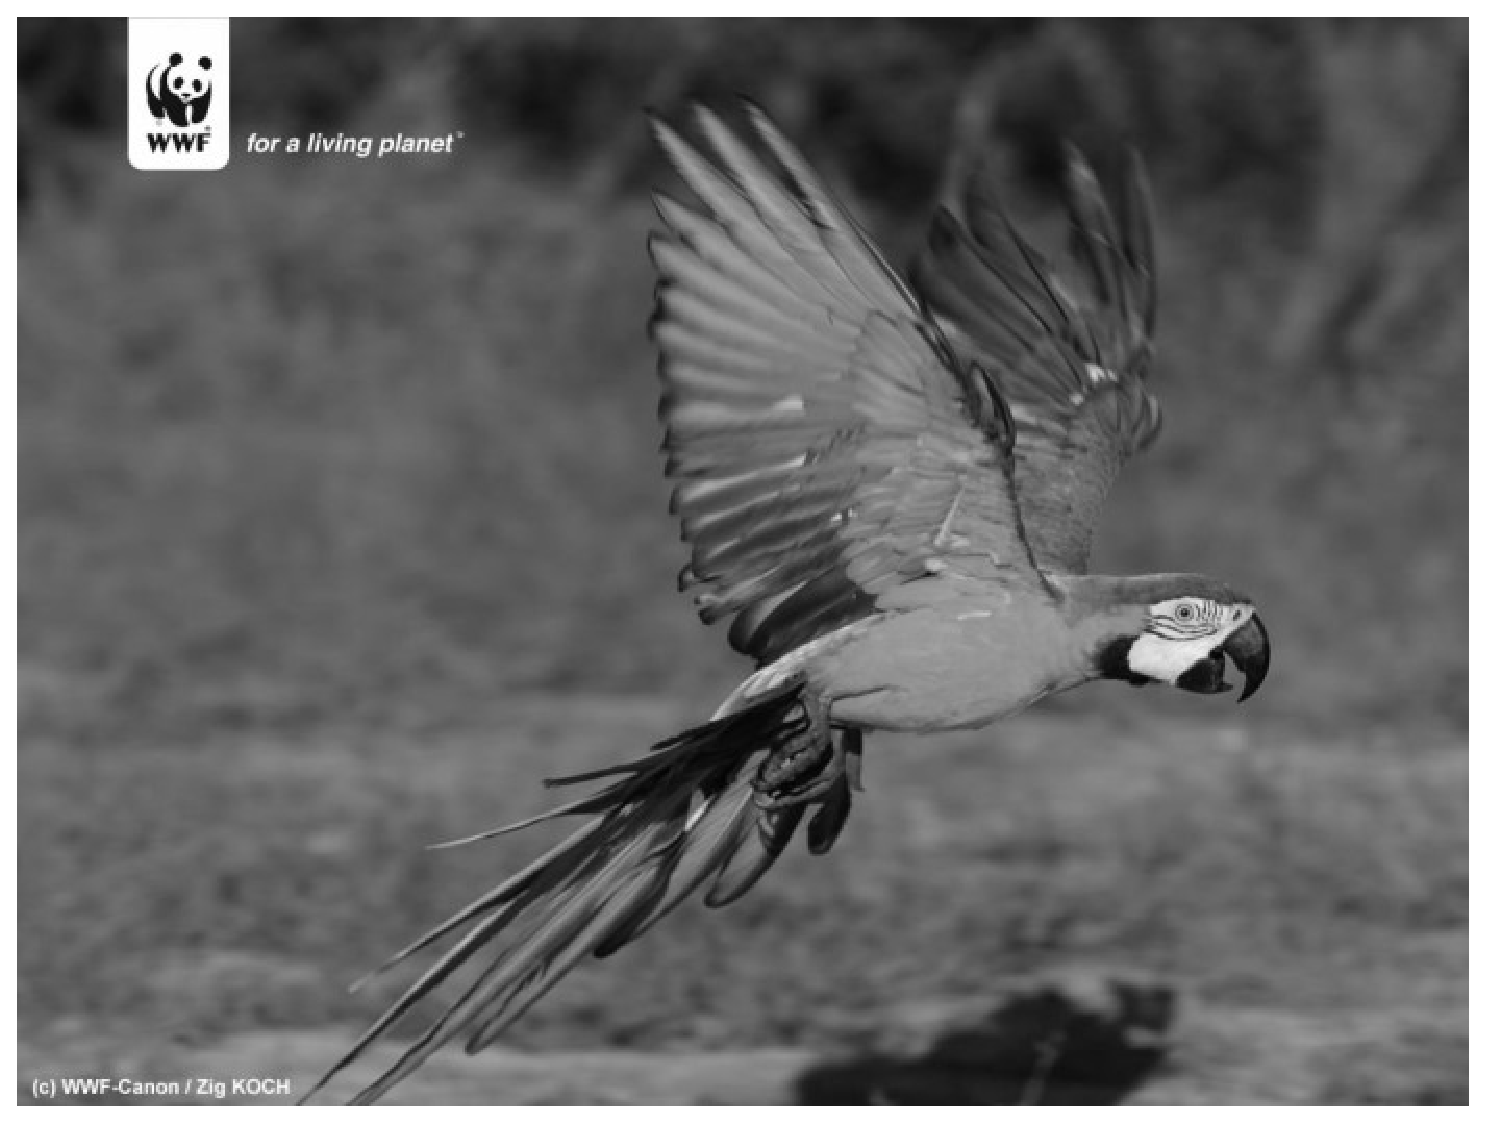
\includegraphics[width = 0.4 \linewidth]{ara_orig.eps}
	    
	    \caption{Image originale}
	\end{figure}
 
\newpage
	
    \begin{Def}[Vecteurs associ\'{e}s \`{a} la transformation par ondelettes de Haar]
      $\phantom{Prop}$ D'apr\`{e}s la remarque pr\'{e}c\'{e}dente, on pose les vecteurs associ\'{e}s \`{a} la transformation par ondelettes de Haar suivants
      \footnote{Rigoureusement il faudrait utiliser le scalaire $ \frac{1}{\sqrt{2}}$, cependant, suite \`{a} des probl\`{e}mes li\'{e}s
	\`{a} l'intensit\'{e} des pixels lors de la compression, apparemment li\'{e}s au choix de ce scalaire, j'ai d\'{e}cid\'{e}
	d'utiliser le scalaire $\frac{1}{2}$. (Voir l'annexe A pour un exemple).}:
      \begin{center}
	$ \mathcal{H}_a \; = \; \frac{1}{2} (1, 1) \; \in \; \mathbb{R}^2 $ pour les espaces $(V_j)_{j \in \mathbb{Z}}$ \\
	$ \mathcal{H}_d \; = \; \frac{1}{2} (1, -1) \; \in \; \mathbb{R}^2 $ pour les espaces $(W_j)_{j \in \mathbb{Z}}$
      \end{center}
    \end{Def}
	
    \begin{Def}[Fonction filtre]
	$\phantom{Prop}$ Soit $ n \in \mathbb{N} $. Soient $ b, x \in \mathbb{R}^n $. Soit $ a \in \mathbb{R}^* $. \newline
	$\phantom{Prop}$ On d\'{e}finit un nouveau vecteur $ y \in \mathbb{R}^n $, image de $x$ par la fonction $ \Phi_{a,b} $ tel que :
	\begin{center}
	  $ \forall i \in [1;n], \; e_k^* (y) \; = \; \frac{1}{a} \displaystyle\sum_{i = 1}^k e_i^* (b) e_{k - i}^* (x) $
	\end{center}
    \end{Def}
	
    \begin{Prop}[Cas particulier de la fonction sur l'espace d'approximation]
	$\phantom{Prop}$ Pour l'algorithme que l'on codera, on consid\'{e}rera la fonction $ \Phi_{1,\mathcal{H}_a} $ tel que 
	pour tout $ x \in \mathbb{R}^n $,
	\begin{center}
	  $ e_1^* (\Phi_{1, \mathcal{H}_a}) \; = \; \frac{1}{2} e_1^* (x) $ \\
	  $ \forall j \in [2;n], e_j^* (\Phi_{1, \mathcal{H}_a}) \; = \; \frac{1}{2}(e_{j - 1}^* (x) + e_j^* (x))$
	\end{center}
	$\phantom{Prop}$ On note alors cette fonction $\varPhi$.
    \end{Prop}

    \begin{Prop}[Cas particulier de la fonction sur l'espace de d\'{e}tails]
	$\phantom{Prop}$ On consid\'{e}rera dans ce cas, la fonction $ \Phi_{1,\mathcal{H}_d} $ tel que 
	pour tout $ x \in \mathbb{R}^n $,
	\begin{center}
	  $ e_1^* (\Phi_{1, \mathcal{H}_d}) \; = \; \frac{1}{2} e_1^* (x) $ \\
	  $ \forall j \in [2;n], e_j^* (\Phi_{1, \mathcal{H}_d}) \; = \; \frac{1}{2}(e_{j - 1}^* (x) + e_j^* (x))$
	\end{center}
	$\phantom{Prop}$ On note alors cette fonction $\varPsi$.
    \end{Prop}
	
    \paragraph{} Avant d'\'{e}tudier l'algorithme, il reste encore \`{a} d\'{e}finir une fonction permettant d'extraire un sous vecteur.
    
    \begin{Def}[Fonction d'\'{e}chantillonage]
	$\phantom{Prop}$ On note $\downarrow_k $, pour $k \in [1;n]$ la fonction suivante :
	\begin{center}
	  $ \downarrow_k \, : \mathbb{R}^n \longrightarrow \mathbb{R}^{\lfloor n / k \rfloor} $ \\
	  $ (x_1, x_2, ..., x_n) \longmapsto (x_k, x_{2 k}, ..., x_{\lfloor n / k \rfloor k}) $
	\end{center}
    \end{Def}

    \paragraph{Algorithme de Mallat} Consid\'{e}rons une image sous forme de matrice $M \in M_{n,m}(\mathbb{R})$, o\`{u} l'on supposera
	que $n$ et $m$ sont deux multiples d'une puissance de $2$, quitte \`{a} la normaliser en ajoutant des z\'{e}ros. \newline
	
	\begin{center}
	
	  \begin{tabular}{| c | c | c | c | c | c | c | c |}
	      \hline
	      $M_{1,1}$ & $M_{1,2}$ & $M_{1,3}$ & $M_{1,4}$ & $M_{1,5}$ & $M_{1,6}$ & $M_{1,7}$ & $M_{1,8}$ \\ 
	      \hline
	      $M_{2,1}$ & $M_{2,2}$ & $M_{2,3}$ & $M_{2,4}$ & $M_{2,5}$ & $M_{2,6}$ & $M_{2,7}$ & $M_{2,8}$ \\ 
	      \hline
	      $M_{3,1}$ & $M_{3,2}$ & $M_{3,3}$ & $M_{3,4}$ & $M_{3,5}$ & $M_{3,6}$ & $M_{3,7}$ & $M_{3,8}$ \\ 
	      \hline
	      $M_{4,1}$ & $M_{4,2}$ & $M_{4,3}$ & $M_{4,4}$ & $M_{4,5}$ & $M_{4,6}$ & $M_{4,7}$ & $M_{4,8}$ \\ 
	      \hline
	      $M_{5,1}$ & $M_{5,2}$ & $M_{5,3}$ & $M_{5,4}$ & $M_{5,5}$ & $M_{5,6}$ & $M_{5,7}$ & $M_{5,8}$ \\ 
	      \hline
	      $M_{6,1}$ & $M_{6,2}$ & $M_{6,3}$ & $M_{6,4}$ & $M_{6,5}$ & $M_{6,6}$ & $M_{6,7}$ & $M_{6,8}$ \\ 
	      \hline
	      $M_{7,1}$ & $M_{7,2}$ & $M_{7,3}$ & $M_{7,4}$ & $M_{7,5}$ & $M_{7,6}$ & $M_{7,7}$ & $M_{7,8}$ \\ 
	      \hline
	      $M_{8,1}$ & $M_{8,2}$ & $M_{8,3}$ & $M_{8,4}$ & $M_{8,5}$ & $M_{8,6}$ & $M_{8,7}$ & $M_{8,8}$ \\  
	      \hline
	  \end{tabular}
	 
	\end{center}
	
	Pour calculer $V_{-j}$ et $W_{-j}$, on applique la fonction filtre en premier lieu sur les lignes de $M$. \newline
	On applique alors les fonctions $ \varPhi $ et $\varPsi$ au vecteur $ M_{i,[1;m/j]} \; = \; (M_{i,1}, M_{i,2}, ..., M_{i, m/j}) $ 
	puis on applique au r\'{e}sultat ainsi obtenu la fonction de sous-\'{e}chantillonage $\downarrow_2$.
	images que l'on notera respectivement $\downarrow_2 \varPhi^i$ et $\downarrow_2 \varPsi^i$
	
\newpage

	Ainsi la nouvelle matrice devient :
	
	
	\begin{center}
	
	  \begin{tabular}{| c | c | c | c || c | c | c | c |}
	      \hline
	      $(\downarrow_2 \varPhi^1)_{1,1}$ & $(\downarrow_2 \varPhi^1)_{1,2}$ & $(\downarrow_2 \varPhi^1)_{1,3}$ & $(\downarrow_2 \varPhi^1)_{1,4}$ 
	      & $(\downarrow_2 \varPsi^1)_{1,1}$ & $(\downarrow_2 \varPsi^1)_{1,2}$ & $(\downarrow_2 \varPsi^1)_{1,3}$ & $(\downarrow_2 \varPsi^1)_{1,4}$ \\ 
	      \hline
	      $(\downarrow_2 \varPhi^2)_{2,1}$ & $(\downarrow_2 \varPhi^2)_{2,2}$ & $(\downarrow_2 \varPhi^2)_{2,3}$ & $(\downarrow_2 \varPhi^2)_{2,4}$ 
	      & $(\downarrow_2 \varPsi^2)_{2,1}$ & $(\downarrow_2 \varPsi^2)_{2,2}$ & $(\downarrow_2 \varPsi^2)_{2,3}$ & $(\downarrow_2 \varPsi^2)_{2,4}$ \\ 
	      \hline
	      $(\downarrow_2 \varPhi^3)_{3,1}$ & $(\downarrow_2 \varPhi^3)_{3,2}$ & $(\downarrow_2 \varPhi^3)_{3,3}$ & $(\downarrow_2 \varPhi^3)_{3,4}$ 
	      & $(\downarrow_2 \varPsi^3)_{3,1}$ & $(\downarrow_2 \varPsi^3)_{3,2}$ & $(\downarrow_2 \varPsi^3)_{3,3}$ & $(\downarrow_2 \varPsi^3)_{3,4}$ \\ 
	      \hline
	      $(\downarrow_2 \varPhi^4)_{4,1}$ & $(\downarrow_2 \varPhi^4)_{4,2}$ & $(\downarrow_2 \varPhi^4)_{4,3}$ & $(\downarrow_2 \varPhi^4)_{4,4}$ 
	      & $(\downarrow_2 \varPsi^4)_{4,1}$ & $(\downarrow_2 \varPsi^4)_{4,2}$ & $(\downarrow_2 \varPsi^4)_{4,3}$ & $(\downarrow_2 \varPsi^4)_{4,4}$ \\ 
	      \hline
	      $(\downarrow_2 \varPhi^5)_{5,1}$ & $(\downarrow_2 \varPhi^5)_{5,2}$ & $(\downarrow_2 \varPhi^5)_{5,3}$ & $(\downarrow_2 \varPhi^5)_{5,4}$ 
	      & $(\downarrow_2 \varPsi^5)_{5,1}$ & $(\downarrow_2 \varPsi^5)_{5,2}$ & $(\downarrow_2 \varPsi^5)_{5,3}$ & $(\downarrow_2 \varPsi^5)_{5,4}$ \\ 
	      \hline
	      $(\downarrow_2 \varPhi^6)_{6,1}$ & $(\downarrow_2 \varPhi^6)_{6,2}$ & $(\downarrow_2 \varPhi^6)_{6,3}$ & $(\downarrow_2 \varPhi^6)_{6,4}$ 
	      & $(\downarrow_2 \varPsi^6)_{6,1}$ & $(\downarrow_2 \varPsi^6)_{6,2}$ & $(\downarrow_2 \varPsi^6)_{6,3}$ & $(\downarrow_2 \varPsi^6)_{6,4}$ \\ 
	      \hline
	      $(\downarrow_2 \varPhi^7)_{7,1}$ & $(\downarrow_2 \varPhi^7)_{7,2}$ & $(\downarrow_2 \varPhi^7)_{7,3}$ & $(\downarrow_2 \varPhi^7)_{7,4}$ 
	      & $(\downarrow_2 \varPsi^7)_{7,1}$ & $(\downarrow_2 \varPsi^7)_{7,2}$ & $(\downarrow_2 \varPsi^7)_{7,3}$ & $(\downarrow_2 \varPhi^7)_{7,4}$ \\ 
	      \hline
	      $(\downarrow_2 \varPhi^8)_{8,1}$ & $(\downarrow_2 \varPhi^8)_{8,2}$ & $(\downarrow_2 \varPhi^8)_{8,3}$ & $(\downarrow_2 \varPhi^8)_{8,4}$ 
	      & $(\downarrow_2 \varPsi^8)_{8,1}$ & $(\downarrow_2 \varPsi^8)_{8,2}$ & $(\downarrow_2 \varPsi^8)_{8,3}$ & $(\downarrow_2 \varPsi^8)_{8,4}$ \\  
	      \hline
	  \end{tabular}
	 
	\end{center}
	
	En deuxi\`{e}me lieu, on applique aux colonnes not\'{e}es $M_{[1;n/j], j}$ de cette nouvelle matrice ces m\^{e}mes fonctions 
	\footnote{La matrice est s\'{e}par\'{e}e en deux uniquement pour plus de lisibilit\'{e}}:
	
	\begin{center}
	  \begin{tabular}{| c | c | c | c |}
	      \hline
	      $(\downarrow_2 (\varPhi $o$ \varPhi)^1)_{1,1}$ & $(\downarrow_2 (\varPhi $o$ \varPhi)^1)_{1,2}$ & $(\downarrow_2 (\varPhi $o$ \varPhi)^1)_{1,3}$ & $(\downarrow_2 (\varPhi $o$ \varPhi)^1)_{1,4}$ \\
	      \hline
	      $(\downarrow_2 (\varPhi $o$ \varPhi)^2)_{2,1}$ & $(\downarrow_2 (\varPhi $o$ \varPhi)^2)_{2,2}$ & $(\downarrow_2 (\varPhi $o$ \varPhi)^2)_{2,3}$ & $(\downarrow_2 (\varPhi $o$ \varPhi)^2)_{2,4}$ \\ 
	      \hline
	      $(\downarrow_2 (\varPhi $o$ \varPhi)^3)_{3,1}$ & $(\downarrow_2 (\varPhi $o$ \varPhi)^3)_{3,2}$ & $(\downarrow_2 (\varPhi $o$ \varPhi)^3)_{3,3}$ & $(\downarrow_2 (\varPhi $o$ \varPhi)^3)_{3,4}$ \\
	      \hline
	      $(\downarrow_2 (\varPhi $o$ \varPhi)^4)_{4,1}$ & $(\downarrow_2 (\varPhi $o$ \varPhi)^4)_{4,2}$ & $(\downarrow_2 (\varPhi $o$ \varPhi)^4)_{4,3}$ & $(\downarrow_2 (\varPhi $o$ \varPhi)^4)_{4,4}$ \\
	      \hline
	      \hline
	      $(\downarrow_2 (\varPsi $o$ \varPhi)^5)_{5,1}$ & $(\downarrow_2 (\varPsi $o$ \varPhi)^5)_{5,2}$ & $(\downarrow_2 (\varPsi $o$ \varPhi)^5)_{5,3}$ & $(\downarrow_2 (\varPsi $o$ \varPhi)^5)_{5,4}$ \\
	      \hline
	      $(\downarrow_2 (\varPsi $o$ \varPhi)^6)_{6,1}$ & $(\downarrow_2 (\varPsi $o$ \varPhi)^6)_{6,2}$ & $(\downarrow_2 (\varPsi $o$ \varPhi)^6)_{6,3}$ & $(\downarrow_2 (\varPsi $o$ \varPhi)^6)_{6,4}$ \\
	      \hline
	      $(\downarrow_2 (\varPsi $o$ \varPhi)^7)_{7,1}$ & $(\downarrow_2 (\varPsi $o$ \varPhi)^7)_{7,2}$ & $(\downarrow_2 (\varPsi $o$ \varPhi)^7)_{7,3}$ & $(\downarrow_2 (\varPsi $o$ \varPhi)^7)_{7,4}$ \\
	      \hline
	      $(\downarrow_2 (\varPsi $o$ \varPhi)^8)_{8,1}$ & $(\downarrow_2 (\varPsi $o$ \varPhi)^8)_{8,2}$ & $(\downarrow_2 (\varPsi $o$ \varPhi)^8)_{8,3}$ & $(\downarrow_2 (\varPsi $o$ \varPhi)^8)_{8,4}$ \\
	      \hline
	  \end{tabular}
	  
	  \vspace{1cm}
	  
	  \begin{tabular}{| c | c | c | c |}
	      \hline
	      $(\downarrow_2 (\varPhi $o$ \varPsi)^1)_{1,1}$ & $(\downarrow_2 (\varPhi $o$ \varPsi)^1)_{1,2}$ & $(\downarrow_2 (\varPhi $o$ \varPsi)^1)_{1,3}$ & $(\downarrow_2 (\varPhi $o$ \varPsi)^1)_{1,4}$ \\ 
	      \hline
	      $(\downarrow_2 (\varPhi $o$ \varPsi)^2)_{2,1}$ & $(\downarrow_2 (\varPhi $o$ \varPsi)^2)_{2,2}$ & $(\downarrow_2 (\varPhi $o$ \varPsi)^2)_{2,3}$ & $(\downarrow_2 (\varPhi $o$ \varPsi)^2)_{2,4}$ \\
	      \hline
	      $(\downarrow_2 (\varPhi $o$ \varPsi)^3)_{3,1}$ & $(\downarrow_2 (\varPhi $o$ \varPsi)^3)_{3,2}$ & $(\downarrow_2 (\varPhi $o$ \varPsi)^3)_{3,3}$ & $(\downarrow_2 (\varPhi $o$ \varPsi)^3)_{3,4}$ \\ 
	      \hline
	      $(\downarrow_2 (\varPhi $o$ \varPsi)^4)_{4,1}$ & $(\downarrow_2 (\varPhi $o$ \varPsi)^4)_{4,2}$ & $(\downarrow_2 (\varPhi $o$ \varPsi)^4)_{4,3}$ & $(\downarrow_2 (\varPhi $o$ \varPsi)^4)_{4,4}$ \\ 
	      \hline
	      \hline
	      $(\downarrow_2 (\varPsi $o$ \varPsi)^5)_{5,1}$ & $(\downarrow_2 (\varPsi $o$ \varPsi)^5)_{5,2}$ & $(\downarrow_2 (\varPsi $o$ \varPsi)^5)_{5,3}$ & $(\downarrow_2 (\varPsi $o$ \varPsi)^5)_{5,4}$ \\ 
	      \hline
	      $(\downarrow_2 (\varPsi $o$ \varPsi)^6)_{6,1}$ & $(\downarrow_2 (\varPsi $o$ \varPsi)^6)_{6,2}$ & $(\downarrow_2 (\varPsi $o$ \varPsi)^6)_{6,3}$ & $(\downarrow_2 (\varPsi $o$ \varPsi)^6)_{6,4}$ \\ 
	      \hline
	      $(\downarrow_2 (\varPsi $o$ \varPsi)^7)_{7,1}$ & $(\downarrow_2 (\varPsi $o$ \varPsi)^7)_{7,2}$ & $(\downarrow_2 (\varPsi $o$ \varPsi)^7)_{7,3}$ & $(\downarrow_2 (\varPsi $o$ \varPsi)^7)_{7,4}$ \\ 
	      \hline
	      $(\downarrow_2 (\varPsi $o$ \varPsi)^8)_{8,1}$ & $(\downarrow_2 (\varPsi $o$ \varPsi)^8)_{8,2}$ & $(\downarrow_2 (\varPsi $o$ \varPsi)^8)_{8,3}$ & $(\downarrow_2 (\varPsi $o$ \varPsi)^8)_{8,4}$ \\  
	      \hline
	  \end{tabular}

	\end{center}
	
\newpage
	
	L'algorithme, pouvant \^{e}tre consid\'{e}r\'{e} comme une fonction not\'{e}e $TW$, 
	pour calculer la transform\'{e}e par ondelettes sur les espaces $V_{-j_V}$ et $W_{-j_V}$ est donc le suivant :
	
	\begin{algorithm}
	  \caption{Transform\'{e}e par ondelettes d'une matrice}
	  
	  \begin{algorithmic}
	    \REQUIRE { une matrice $M \in M_{n,m}(\mathbb{R}) $ et un entier $j_V \in \mathbb{N}$ }
	    \IF {$n$ ne divise pas $2^{j_V}$ } 
	      \STATE {Ajouter $(n \, - \, n \, \% \, 2^{j_V})$ lignes de z\'{e}ros \`{a} $M$} 
	    \ENDIF
	    \IF {$m$ ne divise pas $2^{j_V}$ } 
	      \STATE {Ajouter $(m \, - \, m \, \% \, 2^{j_V})$ colonnes de z\'{e}ros \`{a} $M$} 
	    \ENDIF
	    
	    \FOR { $k = 0$ \TO $j_V - 1$}
	      \FOR { $i = 1$ \TO $n / 2^k$}
		\STATE { Affecter au vecteur $M_{i,[1;\frac{m}{2^{k + 1}}]}$ le r\'{e}sultat de
		  la fonction $ (\downarrow_2 \, $o$ \, \varPhi) $ appliqu\'{e} au vecteur $M_{i,[1;\frac{m}{2^k}]}$ }
		\STATE { Affecter au vecteur $M_{i,[\frac{m}{2^{k + 1}} + 1;\frac{m}{2^k}]}$ le r\'{e}sultat de
		  la fonction $ (\downarrow_2 \, $o$ \, \varPsi) $ appliqu\'{e} au vecteur $M_{i,[1;\frac{m}{2^k}]}$  }
	      \ENDFOR
	      \FOR { $j = 1$ \TO $m / 2^k$}
		\STATE { Affecter au vecteur $M_{[1;\frac{n}{2^{k + 1}}],j}$ le r\'{e}sultat de
		  la fonction $ (\downarrow_2 \, $o$ \, \varPhi) $ appliqu\'{e} au vecteur $M_{[1;\frac{n}{2^k}],j}$ }
		\STATE { Affecter au vecteur $M_{[\frac{n}{2^{k + 1}} + 1;\frac{n}{2^k}],j}$ le r\'{e}sultat de
		  la fonction $ (\downarrow_2 \, $o$ \, \varPsi) $ appliqu\'{e} au vecteur $M_{[1;\frac{n}{2^k}],j}$  }
	      \ENDFOR
	    \ENDFOR
	    \ENSURE {La matrice $M$ ainsi obtenue}
	  \end{algorithmic}

	\end{algorithm}

	Avec l'image t\'{e}moin, on obtient l'image suivante pour $V_{-1}$ i.e. $j_V \, = \, 1$:
	\begin{figure}[!h]
	    \centering
	    
	    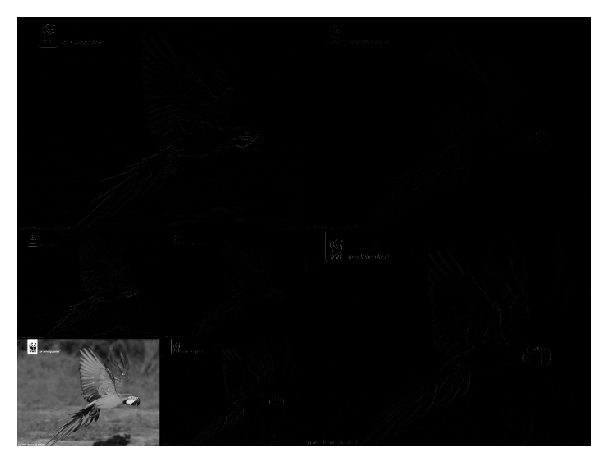
\includegraphics[width = 0.4 \linewidth]{ara_wt_V1.eps}
	    
	    \caption{Transform\'{e}e par ondelettes de l'image t\'{e}moin pour $j_V \, = \, 1$}
	\end{figure}
	
\newpage
	
	\paragraph{} Suite \`{a} l'application de l'algorithme pour $j_V \in \mathbb{N}$, on obtient une matrice de la forme :
	
	\vspace{6cm}
	
	  \begin{figure}[!h]
	      \centering
	      
	      \begin{pspicture}(0,0)(0,0)

		\psframe[linewidth=2pt](-6,-6)(6,6)
		
		\psline[linewidth=1.5pt,linecolor=green](0,6)(0,0)
		\psline[linewidth=1.5pt,linecolor=green](-6,0)(0,0)
		\psline[linestyle=dotted](0,0)(0,-6)
		\psline[linestyle=dotted](0,0)(6,0)
		\rput(3,3){\large {\textcolor{green}{$W_{-1}$}}}
		\rput(3,-3){\large {\textcolor{green}{$W_{-1}$}}}
		\rput(-3,-3){\large {\textcolor{green}{$W_{-1}$}}}
		\rput(-2.8,2.8){\large {\textbf{\textcolor{green}{$V_{-1}$}}}}
		
		\psline[linewidth=1.5pt,linecolor=blue](-3,6)(-3,3)
		\psline[linewidth=1.5pt,linecolor=blue](-6,3)(-3,3)
		\psline[linestyle=dotted](-3,3)(-3,0)
		\psline[linestyle=dotted](-3,3)(0,3)
		\rput(-1.5,1.5){\large {\textcolor{blue}{...}}}
		\rput(-1.5,4.5){\large {\textcolor{blue}{...}}}
		\rput(-4.5,1.5){\large {\textcolor{blue}{...}}}
		\rput(-4.2,4.3){\large {\textbf{\textcolor{blue}{$V_{- (j_V - 1)}$}}}}
		
		\psline[linewidth=1.5pt,linecolor=red](-4.5,6)(-4.5,4.5)
		\psline[linewidth=1.5pt,linecolor=red](-6,4.5)(-4.5,4.5)
		\psline[linestyle=dotted](-4.5,4.5)(-4.5,3)
		\psline[linestyle=dotted](-4.5,4.5)(-3,4.5)
		\rput(-5.25,5.25){\large {\textbf{\textcolor{red}{$V_{-j_V}$}}}}
		\rput(-5.25,3.75){\large {\textcolor{red}{$W_{-j_V}$}}}
		\rput(-3.75,5.25){\large {\textcolor{red}{$W_{-j_V}$}}}
		\rput(-3.75,3.75){\large {\textcolor{red}{$W_{-j_V}$}}}
		
	      \end{pspicture}
	      
	      \vspace{6cm}
	      
	      \caption{Sch\'{e}ma de la matrice issue de l'algorithme pr\'{e}c\'{e}dent pour $j_V \in \mathbb{N}$}	   
	  \end{figure}

    \begin{Def}[Fonction de dilatation]
	$\phantom{Prop}$ On note $\uparrow_2 $ la fonction suivante :
	\begin{center}
	  $ \uparrow_2 \, : \mathbb{R}^n \longrightarrow \mathbb{R}^{2 n} $ \\
	  $ (x_1, x_2, ..., x_n) \longmapsto (x_1,0, x_2, 0, ..., 0, x_n) $
	\end{center}
    \end{Def}

    \begin{Def}[Vecteurs associ\'{e}s \`{a} la reconstruction]
      $\phantom{Prop}$ D'apr\`{e}s la remarque pr\'{e}c\'{e}dente, on pose les vecteurs associ\'{e}s \`{a} la reconstruction suivants :
      \begin{center}
	$ \mathcal{R}_a \; = \; (1, 1) \; \in \; \mathbb{R}^2 $ pour les espaces $(V_j)_{j \in \mathbb{Z}}$ \\
	$ \mathcal{R}_d \; = \; (1, -1) \; \in \; \mathbb{R}^2 $ pour les espaces $(V_j)_{j \in \mathbb{Z}}$
      \end{center}
    \end{Def}
    
    \begin{Def}[Fonctions filtres associ\'{e}s \`{a} la reconstruction]
      $\phantom{Prop}$ De mani\`{e}re similaire aux fonctions filtres d\'{e}finies dans les propri\'{e}t\'{e}s $8$ et $9$, 
      on d\'{e}finit les fonctions filtres de reconstruction suivantes :
      \begin{center}
	$ \varGamma \, = \, \Phi_{1, \mathcal{R}_a} $ \\
	$ \varOmega \, = \, \Phi_{1, \mathcal{R}_b} $
      \end{center}

    \end{Def}

\newpage

    \paragraph{} D'apr\`{e}s la d\'{e}finition 6, comme $ \forall j \in \mathbb{Z}, V_{j - 1} \, = \, V_j \displaystyle \bigoplus^\perp W_j $, on en 
	d\'{e}duit l'algorithme de reconstruction, pouvant \^{e}tre consid\'{e}r\'{e} comme une fonction not\'{e}e $R$, suivant :
    
    \begin{algorithm}
      \caption{Reconstruction d'une matrice}
      
      \begin{algorithmic}
	\REQUIRE { une matrice $M \in M_{n,m}(\mathbb{R}) $ et un entier $j_V \in \mathbb{N}$ }	
	\FOR { $k = j_V - 1$ \TO $0$}
	  \FOR { $j = 1$ \TO $m / 2^k$}
	    \STATE { Affecter au vecteur $M_{[1;\frac{n}{2^k}],j}$  la somme du r\'{e}sultat de la fonction 
		$ (\varGamma \, $o$ \, \uparrow_2) $ appliqu\'{e}e au vecteur $M_{[1;\frac{n}{2^{k + 1}}],j}$ 
		et du r\'{e}sultat de la fonction $ (\varOmega \, $o$ \, \uparrow_2) $ appliqu\'{e}e au vecteur
		$M_{[\frac{n}{2^{k + 1}} + 1;\frac{n}{2^k}],j}$ }
	  \ENDFOR
	  \FOR { $i = 1$ \TO $n / 2^k$}
	    \STATE { Affecter au vecteur $M_{i,[1;\frac{m}{2^{k}}]}$  la somme du r\'{e}sultat de la fonction 
		$ (\varGamma \, $o$ \, \uparrow_2) $ appliqu\'{e}e au vecteur $M_{i,[1;\frac{m}{2^{k + 1}}]}$ 
		et du r\'{e}sultat de la fonction $ (\varOmega \, $o$ \, \uparrow_2) $ appliqu\'{e}e au vecteur
		$M_{i,[\frac{m}{2^{k + 1}} + 1;\frac{m}{2^k}]}$  }
	  \ENDFOR
	\ENDFOR
	\ENSURE {La matrice $M$ ainsi obtenue}
      \end{algorithmic}

    \end{algorithm}
    
    \begin{Rem}
      La somme mentionn\'{e}e permet de passer de deux vecteurs $(x_1, x_2, .., x_n)$ et $(y_1, y_2, ... y_n)$ 
      au vecteur $(x_1, y_1, x_2, y_2, ..., x_n, y_n)$.
    \end{Rem}

    
    \begin{Prop}
      $\phantom{Prop}$ Soit $j \in \mathbb{N}$. La fonction $TW_j$ est inversible et $R_j \; = (TW_j)^{-1}$.
    \end{Prop}
    
    \begin{Dem}
      $\phantom{Prop}$ Soit $(x, y) \in \mathbb{R}^2$.
      Par d\'{e}finition des algorithmes, il s'agit en fait de d\'{e}montrer que :
      
      \begin{center}
	$ \Phi_{1, \mathcal{R}_a} \Big(\Phi_{1, \mathcal{H}_a}(x, y), \Phi_{1, \mathcal{H}_d}(x, y) \Big) \; = \; x $ \\
	$ \Phi_{1, \mathcal{R}_d} \Big(\Phi_{1, \mathcal{H}_a}(x, y), \Phi_{1, \mathcal{H}_d}(x, y) \Big) \; = \; y $
      \end{center}
      
      $\phantom{Prop}$ C'est \`{a} dire, par d\'{e}finition des fonctions filtres, qu'il s'agit de montrer que :
      
      \begin{center}
	$ \frac{x + y}{2} + \frac{x - y}{2} \; = \; x $ \\
	$ \frac{x + y}{2} - \frac{x - y}{2} \; = \; y $
      \end{center}
      
      $\phantom{Prop}$ Ce qui est clairement le cas.

    \end{Dem}

    
    \paragraph{} Avec l'image pr\'{e}c\'{e}dente (figure $4$) issue de $TW_1$, en lui appliquant la fonction $R_1$, on obtient :
    
      \begin{figure}[!h]
	    \centering
	    
	    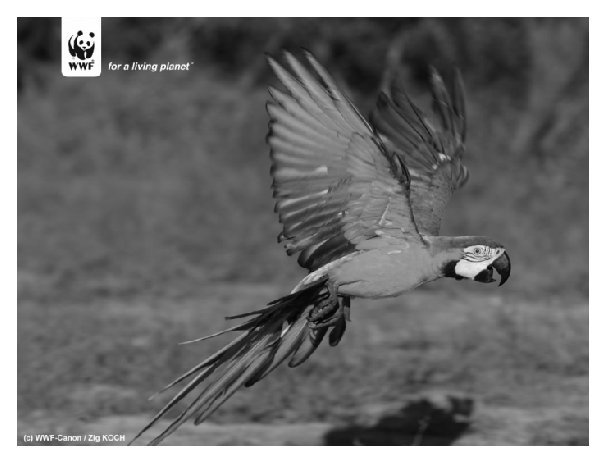
\includegraphics[width = 0.4 \linewidth]{ara_decomp.eps}
	    
	    \caption{Recomposition de l'image figure $4$}
      \end{figure}
      $\phantom{Prop}$ Il s'agit bien l\`{a} de l'image originale $\phantom{ }$ !

\newpage

\section*{III. Un algorithme efficace ?}

  \subsection*{1) \'{E}tude de la complexit\'{e}}
    
    \begin{Prop}[Complexit\'{e} de la fonction $TW$]
      $\phantom{Prop}$ Soit $j_V \in \mathbb{N}$. Pour une image de taille $n$x$m$ pixels, la complexit\'{e} de $TW_{j_V}$ est :
      \begin{center}
	$ \boxed{O \Big(nm + n m^2 + m n^2 \Big)} $
      \end{center}

    \end{Prop}
    
    \begin{Dem}
	$\phantom{Prop}$ Soit $j_V \in \mathbb{N}$. Soit $M \in M_{n,m}(\mathbb{R})$. \\
	$\phantom{Prop}$ La complexit\'{e} de la normalisation est de l'ordre de $O (nm) $. \\
	$\phantom{Prop}$ Soit $k \in [0; j_v - 1]$. Soit $i \in [1;n/2^k]$ \\
	$\phantom{Prop}$ Comme la complexit\'{e} de l'affectation est lin\'{e}aire en la taille du vecteur,
	l'affectation a une complexit\'{e} de $ \frac{m}{2^{k + 1}} - 1 + 1 \; = \; \frac{m}{2^{k+1}}$.\\
	$\phantom{Prop}$ De plus, la fonction $ \downarrow_2 \; $o$ \; \varPhi $ s'effectue en un temps quadratique en la taille du vecteur 
	(due \`{a} la fonction filtre).\\
	$\phantom{Prop}$ Ainsi, le calcul du r\'{e}sultat de cette fonction appliqu\'{e} au vecteur $M_{i, [1;\frac{m}{2^k}]}$ a une 
	complexit\'{e} de $C (\frac{m}{2^k})^2$ avec $C > 0$. \\
	$\phantom{Prop}$ Or 
	\begin{eqnarray}
	  2 \displaystyle \sum_{i = 1}^{n/2^k} \Big( \frac{m}{2^{k+1}} + C\frac{m^2}{2^{2k}} \Big) & = &
	  2 \Big( \frac{m}{2^{k+1}} + C\frac{m^2}{2^{2k}} \Big) \Big( \frac{n}{2^k} - 1 + 1 \Big) \\
	  & = & C \frac{n m^2}{2^{3k - 1}} + \frac{nm}{2^{2k}} 
	\end{eqnarray}

	Ainsi, la premi\`{e}re boucle s'effectue en $ O \Big(\frac{n m^2}{2^{3k - 1}} \Big) $. \\
	On d\'{e}montre de m\^{e}me que la deuxi\`{e}me boucle s'effectue en $ O \Big(\frac{m n^2}{2^{3k - 1}} \Big) $. \\
	
	$\phantom{Prop}$ Bilan : (les nombres $C_1$, $C_2$ et $C_3$ sont des r\'{e}els strictements positifs et sont associ\'{e}s aux $O$)
	\begin{eqnarray}
	  C_1 nm + \displaystyle \sum_{k = 0}^{j_V - 1} \Big( C_2 \frac{n m^2}{2^{3k - 1}} + C_3 \frac{m n^2}{2^{3k - 1}} \Big) & = &
	  C_1 nm + 2 (C_2 n m^2 + C_3 m n^2) \displaystyle \sum_{k = 0}^{j_V - 1} \Big( \frac{1}{2^3} \Big)^k \\
	  & = & C_1 nm + 2 (C_2 n m^2 + C_3 m n^2) \frac{ 1 - (\frac{1}{8})^{j_V} }{ 1 - \frac{1}{8} } \\
	  & = & C_1 nm + 2 (C_2 n m^2 + C_3 m n^2) \frac{ 8 - (\frac{1}{8})^{j_V - 1} }{ 7 } \\
	  & = & C_1 nm + \frac{2}{7} \Big(C_2 n m^2 + C_3 m n^2 \Big) \Bigg( 8 - \bigg(\frac{1}{8} \bigg)^{j_V - 1} \Bigg) \\
	  & \leqslant & C_1 nm + \frac{16}{7} \Big(C_2 n m^2 + C_3 m n^2 \Big)
	\end{eqnarray}
	
	Ainsi la complexit\'{e} de cet algorithme est bien de $ \boxed{O \Big(nm + n m^2 + m n^2 \Big)} $
    
    \end{Dem}
    
    \begin{Rem}
      $\phantom{Prop}$ En utilisant les r\'{e}sultats des propri\'{e}t\'{e}s $8$ et $9$ on peut modifier la fonction $filter$ 
      pour faire chuter cette complexit\'{e} \`{a} $ O(nm) $. Cependant cette modification serait valable uniquement pour les
      ondelettes de Haar.
    \end{Rem}

    
\newpage

    \paragraph{} Voici quelques performances en temps de l'algorithme $TW_{j_V}$ pour des matrices carr\'{e}es 
      (l'image d'origine est la m\^{e}me, seule diff\`{e}re la taille). 
      Les calculs se sont fait avec la configuration suivante :
      \begin{itemize}
       \item[-] CPU : Intel Code 2 CPU 2.40 GHz
       \item[-] RAM : 3.6 Go
      \end{itemize}

    
    \begin{figure}[!h]
	\centering
	
	\vspace{2cm}
      
	\begin{pspicture}(-0.5,-0.5)(11,7)
	  \psset{algebraic=true}
	  \psset{xunit = 1.2cm, yunit = 1.2cm}
	  \psaxes{->}(0,0)(-0.5,-0.5)(11,7)
	  
	  \psdots[linecolor=red](1,0.0055)(2,0.0411)(3,0.136)(4,0.321)(5,0.6244)%
		(6,1.067)(7,1.6947)(8,2.5231)(9,3.5803)(10,4.8928)
	  \psdots[linecolor=blue](1,0.00640973999999999933)(2,0.0472819300000000098)(3,0.158144239999999989)(4,0.368943820000000073)(5, 0.719338689999999872)%
		(6,1.22508318)(7,1.93011454999999955)(8,2.89190439999999967)(9,4.04355051)(10, 5.62726277)
	  \psdots[linecolor=green](1,0.00726497999999992317)(2,0.0483472499999993488)(3,0.167200649999997495)(4, 0.376833849999995891)(5,0.747511669999999)%
		(6,1.25121006000000079)(7,2.02503736999999774)(8,2.89439399000000321)(9,4.16871241000000282)(10,5.62712419999999838)

		
	  \psplot[linecolor=red,linewidth=0.5pt]{0}{10}{(0.47*x^3 + 0.2*x^2)/100}
	  
	  \psline[linestyle=dotted,linewidth=0.5pt](0,1)(11,1)
	  \psline[linestyle=dotted,linewidth=0.5pt](0,2)(11,2)
	  \psline[linestyle=dotted,linewidth=0.5pt](0,3)(11,3)
	  \psline[linestyle=dotted,linewidth=0.5pt](0,4)(11,4)
	  \psline[linestyle=dotted,linewidth=0.5pt](0,5)(11,5)
	  \psline[linestyle=dotted,linewidth=0.5pt](0,6)(11,6)
	  
	  \psline[linestyle=dotted,linewidth=0.5pt](1,0)(1,7)
	  \psline[linestyle=dotted,linewidth=0.5pt](2,0)(2,7)
	  \psline[linestyle=dotted,linewidth=0.5pt](3,0)(3,7)
	  \psline[linestyle=dotted,linewidth=0.5pt](4,0)(4,7)
	  \psline[linestyle=dotted,linewidth=0.5pt](5,0)(5,7)
	  \psline[linestyle=dotted,linewidth=0.5pt](6,0)(6,7)
	  \psline[linestyle=dotted,linewidth=0.5pt](7,0)(7,7)
	  \psline[linestyle=dotted,linewidth=0.5pt](8,0)(8,7)
	  \psline[linestyle=dotted,linewidth=0.5pt](9,0)(9,7)
	  \psline[linestyle=dotted,linewidth=0.5pt](10,0)(10,7)

	\end{pspicture}
	  
	\caption{Complexit\'{e} de la fonction $TW_{j_V}$ (en x$\frac{1}{100} s$) en fonction de la taille de la matrice (x$\frac{1}{100}$)
	  (en rouge $j_V = 1$, en bleu $j_V = 2$ et en vert $j_V = 3$). La courbe rouge a pour \'{e}quation $y = 0.47 x^3 + 0.2 x^2 $. }
    \end{figure}

  \subsection*{2) Compression par ondelettes}
  
    \begin{Nota}[Nombre d'octets d'une image]
      $\phantom{Prop}$ On notera dans la suite $No$ la fonction qui renvoie le nombre d'octets d'une image.
    \end{Nota}

    \begin{Rem}
      $\phantom{Prop}$ Dans toute la suite, on confondra image et matrice.
    \end{Rem}
  
    \paragraph{} On remarque que la transform\'{e}e par ondelettes ne diminue pas la taille en octets de l'image originale.
      Il faut donc trouver une solution permettant de diminuer la taille tout en gardant le maximum d'information contenue 
      dans l'image ayant subie la fonction $TW_{j_V}$ avec $j_V \in \mathbb{N}$.
      
    \paragraph{} L'id\'{e}e est alors d'obtenir deux fichiers, un contenant l'image approxim\'{e}e sur $V_{-j_V}$ et l'autre contenant
      les coefficients des d\'{e}tails non nuls (on stockera valeur et place sous cette forme : $ligne \; colonne \; valeur$
      de type $(int \, * \, int \, * int)$ ). 
      Comme la majorit\'{e} des coefficients contenus dans les espaces de d\'{e}tails $W_{-j}$
      pour $j \in [1;j_V]$ sont nuls, la taille du deuxi\`{e}me fichier et n\'{e}cessairement plus basse.
      
    \begin{Def}[Fonction de compression]
      $\phantom{Prop}$ Ainsi on d\'{e}finit la fonction de compression pour $j_V \in \mathbb{N}$ comme mentionn\'{e} ci-dessus :
      \begin{center}
	$ \gamma_{j_V} : M_{n, m}(\mathbb{R}) \longrightarrow M_{n / 2^{j_V + 1}, m / 2^{j_V + 1}}(\mathbb{R}) $
      \end{center}
      $\phantom{Prop}$ O\`{u} les entiers $n$ et $m$ sont suppos\'{e}s \^{e}tre des puissances de $2$.
    \end{Def}
    
\newpage
  
    \begin{Def}[Taux de compression]
      $\phantom{Prop}$ Soit $j_V \in \mathbb{N}$. On d\'{e}finit alors la fonction taux de compression not\'{e}e $\tau_C$ tel que :
      
      \begin{center}
	$ \tau_C :  M_{n,m}(\mathbb{R}) \longrightarrow [0;1] $ \\
	$ e \longmapsto \frac{No(\gamma_{j_V}(e))}{No(e)} $
      \end{center}

    \end{Def}
    
    \paragraph{} Ainsi, on peut tracer le graphique suivant repr\'{e}sentant le taux de compression $\tau_C$ 
	o\`{u} $it$ repr\'{e}sente l'entier $j_V$. Les images utilis\'{e}es sont carr\'{e}es.

    \begin{figure}[!h]
	\centering
	
	\vspace{6cm}
      
	\begin{pspicture}(-0.5,-0.1)(11,1)
	  \psset{algebraic=true}
	  \psset{xunit = 1.2cm, yunit = 7cm}
	  \psaxes[Dy = 0.1]{->}(0,0)(-0.5,-0.1)(11,1)
	  
	  \psdots[linecolor=red](1,0.7565715046)(2,0.5676195712)(4,0.4373174685)(5,0.4580656859)%
		(6,0.4305469912)(7,0.3791663435)(8,0.3571399554)(9,0.3212047963)(10,0.3130303655)
	  \psdots[linecolor=blue](1,0.7084248353)(2,0.4827244407)(4,0.3227366088)(5,0.3377476822)%
		(6,0.307552215)(7,0.2477460012)(8,0.2106737623)(9,0.1727130344)(10,0.1575234979)
	  \psdots[linecolor=green](1,0.763692021)(2,0.4714878305)(4,0.3000412454)(5,0.3246459588)%
		(6,0.2822794045)(7,0.228303178)(8,0.1817495758)(9,0.149135369)(10,0.1254197424)
	  
	  \psline[linestyle=dotted,linewidth=0.5pt](0,0.1)(11,0.1)
	  \psline[linestyle=dotted,linewidth=0.5pt](0,0.2)(11,0.2)
	  \psline[linestyle=dotted,linewidth=0.5pt](0,0.3)(11,0.3)
	  \psline[linestyle=dotted,linewidth=0.5pt](0,0.4)(11,0.4)
	  \psline[linestyle=dotted,linewidth=0.5pt](0,0.5)(11,0.5)
	  \psline[linestyle=dotted,linewidth=0.5pt](0,0.6)(11,0.6)
	  \psline[linestyle=dotted,linewidth=0.5pt](0,0.7)(11,0.7)
	  \psline[linestyle=dotted,linewidth=0.5pt](0,0.8)(11,0.8)
	  \psline[linestyle=dotted,linewidth=0.5pt](0,0.9)(11,0.9)
	  
	  \psline[linestyle=dotted,linewidth=0.5pt](1,0)(1,1)
	  \psline[linestyle=dotted,linewidth=0.5pt](2,0)(2,1)
	  \psline[linestyle=dotted,linewidth=0.5pt](3,0)(3,1)
	  \psline[linestyle=dotted,linewidth=0.5pt](4,0)(4,1)
	  \psline[linestyle=dotted,linewidth=0.5pt](5,0)(5,1)
	  \psline[linestyle=dotted,linewidth=0.5pt](6,0)(6,1)
	  \psline[linestyle=dotted,linewidth=0.5pt](7,0)(7,1)
	  \psline[linestyle=dotted,linewidth=0.5pt](8,0)(8,1)
	  \psline[linestyle=dotted,linewidth=0.5pt](9,0)(9,1)
	  \psline[linestyle=dotted,linewidth=0.5pt](10,0)(10,1)

	\end{pspicture}
	
	\vspace{1cm}
	  
	\caption{Taux de compression $\tau_C$ en fonction de la taille de la matrice (x$\frac{1}{100}$)
	  (en rouge $j_V = 1$, en bleu $j_V = 2$ et en vert $j_V = 3$) }
    \end{figure}
    
    \begin{Rem}
      $\phantom{Prop}$ Ainsi, d'apr\`{e}s ce graphique, m\^{e}me si le temps recquis est long, la compression semble plus efficace 
	pour les grandes images que pour les petites. De plus, plus $j_V$ augmente, plus la compression est efficace (en effet,
	on divise \`{a} chaque fois la taille de l'image par 2).
    \end{Rem}

    
  \subsection*{3) Estimation de l'erreur}
  
    \paragraph{} Comme on l'a vu dans la partie pr\'{e}c\'{e}dente, la fonction $\gamma$ introduit une erreur qui provient du fait 
	du passage d'une matrice de type $float$ au type $int$. De plus, l'appel \`{a} la fonction $Pixel\_matrix.intmatrix\_of\_matrix$
	introduit une autre erreur qui est le passage d'un intervalle de $\mathbb{R}$ \`{a} l'ensemble $[0;255]$.
	Cependant, on le verra plus tard, le changement de signe n'influe pas sur le calcul de l'erreur.
	
    \paragraph{} On va donc introduire une fonction erreur. Pour cela, l'id\'{e}e la plus simple est d'utiliser une fonction distance.
	Cette fonction distance devra respecter deux crit\`{e}res :
	\begin{itemize}
	 \item [-] prendre en compte la taille de la matrice
	 \item [-] prendre en compte tous les \'{e}carts relatifs entre les coefficients
	\end{itemize}

	
    \begin{Prop}[Distance de compression]
      $\phantom{Prop}$ On d\'{e}finit par cons\'{e}quent la distance suivante :
      \begin{center}
	$d : M_{n,m}(\mathbb{R}) \, $x$ \, M_{n,m}(\mathbb{R}) \longrightarrow \mathbb{R}^+ $ \\
	$ (M, N) \longmapsto \frac{\parallel M - N \parallel}{n m} $
      \end{center}

    \end{Prop}
    
\newpage

    \begin{Def}[Fonction erreur]
      $\phantom{Prop}$ Soit $j_V \in \mathbb{N}$. On d\'{e}finit la fonction erreur comme suit :
      \begin{center}
	$\mathcal{E}_{j_V} : M_{n,m}(\mathbb{R}) \longrightarrow \mathbb{R}  $ \\
	$M \longmapsto d \Bigg(M, \Big((\gamma_{j_V})^{-1} \, $o$ \, \gamma_{j_V}\Big)(M) \Bigg)$
      \end{center}

    \end{Def}
    
    \paragraph{} En reprenant l'image originale, on obtient alors :

      \begin{figure}[!h]

	\begin{tabular}{cc}
	
	  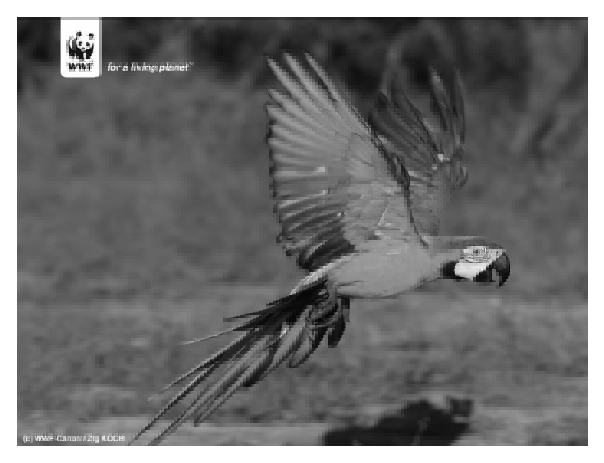
\includegraphics[width = 0.5 \linewidth]{decomp_ara.eps} &
	  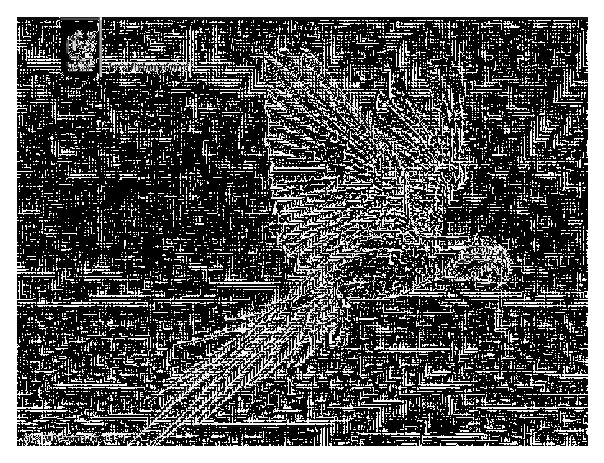
\includegraphics[width = 0.5 \linewidth]{error_ara.eps} \\	
	  
	\end{tabular}
	
	\caption{Image d\'{e}compress\'{e}e issue de $\Big((\gamma_{j_V})^{-1} \, $o$ \, \gamma_{j_V}\Big)$ (\`{a} gauche) et
	    image repr\'{e}sentant l'erreur commise (\`{a} droite)}
	
      \end{figure}  
      

    \begin{figure}[!h]
	\centering
	
	\vspace{4cm}
      
	\begin{pspicture}(-0.5,-0.1)(11,4)
	  \psset{algebraic=true}
	  \psset{xunit = 1.2cm, yunit = 2cm}
	  \psaxes{->}(0,0)(-0.5,-0.1)(11,4)
	  
	  \psdots[linecolor=red](1,1.481759)(2,0.51285625)(4,0.2670741875)(5,0.26985776)%
		(6,0.24228625)(7,0.159483714286)(8,0.141761125)(9,0.082117012346)(10,0.07686232)
	  \psdots[linecolor=blue](1,3.000353)(2,1.49024025)(4,0.7517214375)(5,0.6999072)%
		(6,0.659101027778)(7,0.496295510204)(8,0.3707885625)(9,0.293008506173)(10,0.2368209)
	  \psdots[linecolor=green](2,3.33641325)(4,1.7151745625)(5,2.37448676)%
		(6,1.405078666667)(7,1.718149591837)(8,0.91170034375)(9,1.230958432099)(10,0.66626124)

	  
	  \psline[linestyle=dotted,linewidth=0.5pt](0,1)(11,1)
	  \psline[linestyle=dotted,linewidth=0.5pt](0,2)(11,2)
	  \psline[linestyle=dotted,linewidth=0.5pt](0,3)(11,3)
	  
	  \psline[linestyle=dotted,linewidth=0.5pt](1,0)(1,4)
	  \psline[linestyle=dotted,linewidth=0.5pt](2,0)(2,4)
	  \psline[linestyle=dotted,linewidth=0.5pt](3,0)(3,4)
	  \psline[linestyle=dotted,linewidth=0.5pt](4,0)(4,4)
	  \psline[linestyle=dotted,linewidth=0.5pt](5,0)(5,4)
	  \psline[linestyle=dotted,linewidth=0.5pt](6,0)(6,4)
	  \psline[linestyle=dotted,linewidth=0.5pt](7,0)(7,4)
	  \psline[linestyle=dotted,linewidth=0.5pt](8,0)(8,4)
	  \psline[linestyle=dotted,linewidth=0.5pt](9,0)(9,4)
	  \psline[linestyle=dotted,linewidth=0.5pt](10,0)(10,4)

	\end{pspicture}
	
	\vspace{1cm}
	  
	\caption{Erreur $ \mathcal{E}_{j_V} $ li\'{e}e \`{a} la compression (x$\frac{1}{100}$) en fonction de la taille de la matrice (x$\frac{1}{100}$)
	  (en rouge $j_V = 1$, en bleu $j_V = 2$ et en vert $j_V = 3$) }
    \end{figure}

\newpage

\section*{Conclusion}

  \paragraph{} Ainsi, l'algorithme de Mallat permet de transformer une image par ondelettes. Lorsque cette transformation est faite,
      comme le poids de l'image ne change pas, il a \'{e}t\'{e} n\'{e}cessaire de trouver une solution afin de pouvoir effectivement
      compresser une image. Cette solution produit deux fichiers, ainsi n\'{e}cessaire lors de la transmission de ces donn\'{e}es.
      Peut \^{e}tre serait-il possible d'utiliser la st\'{e}ganographie (autre domaine d'application des ondelettes) afin de r\'{e}cup\'{e}rer 
      plus qu'un seul fichier. De plus, l'image produite par la compression \`{a} diminu\'{e}e de taille, on pourrait donc utiliser une 
      fonction permettant de doubler sa taille en copiant les pixels.
      
  \paragraph{} On a \'{e}galement vu que l'algorithme de Mallat n'introduit pas d'erreur, c'est uniquement d\^{u} \`{a} la conversion
      d'une matrice de type $float$ au type $int$ que l'erreur est introduite. De plus, cette erreur diminue lorsque la taille de l'image
      augmente. Tout comme le taux de compression. Cependant, la complexit\'{e} temporelle est un s\'{e}rieux frein, m\^{e}me si une 
      complexit\'{e} de l'ordre de $O(n^3)$ est acceptable pour un algorithme travaillant sur les matrices. En effet, la transformation
      requiert la plupart des coefficients de la matrice et la fonction $filter$ s'effectue en temps quadratique (que l'on pourrait
      diminuer en un temps lin\'{e}aire dans le cas de l'ondelette de Haar). En titre de comparaison, la complexit\'{e} du produit matriciel
      na\"{i}f (c'est \`{a} dire, l'algorithme issue de la d\'{e}finition) a une complexit\'{e} de $O(n^3)$.
      
  \paragraph{} Enfin, lorsque l'on augmente le nombre d'it\'{e}rations de l'algorithme de Mallat (i.e. le nombre $j_V$),
      le taux de compression augmente mais l'erreur \'{e}galement. Il est donc peut \^{e}tre profitable de rester dans des petites
      valeurs de $j_V$ afin de garder l'int\'{e}grit\'{e} et la coh\'{e}sion des images.
      
  \paragraph{} Par cons\'{e}quent, l'algorithme propos\'{e} ici est plus efficace pour les grandes images plut\^{o}t que les petites, 
      m\^{e}me si l'algorithme s'effectue dans un temps plus long. Il faut donc trouver un compromis pour chaque taille d'image.
      Cependant, les probl\'{e}matiques actuelles de compression concernent surtout les grandes images et non les petites. 
      Finalement, on peut aussi remarquer que cet algorithme est utilis\'{e} pour le format JPEG2000.

\newpage

  \begin{thebibliography}{1}
    \bibitem{comp}
      Pascal \textsc{Szacherski},
      \emph{Compression, ondelettes et algorithmes aff\'{e}rents},
      Janvier 2008
      
    \bibitem{ond}
      Phillip \textsc{K. Poon},
      \emph{Wavelets},
      College of Optical Sciences, University of Arizona,
      2012
      
    \bibitem{matlab}
      Philippe \textsc{Carr\'{e}} et R\'{e}mi \textsc{Cornillet},
      \emph{Code Matlab},
      respectivements professeur de l'universit\'{e} de Poitiers et responsable de l'\'{e}quipe Icones,
      \'{e}tudiant \`{a} l'\'{E}cole Normale Sup\'{e}rieure de Rennes

    \bibitem{twt}
      Ren\'{e} Alt,
      \emph{La transformation en ondelettes},
      Professeur \`{a} l'universit\'{e} Pierre et Marie Curie
    
    \bibitem{ond2}
      Olivier Rioul,
      \emph{Ondelettes r\'{e}guli\`{e}res: application \'{a} la compression d'images fixes},
      T\'{e}l\'{e}com ParisTech, 1993
      
    \bibitem{bmp}
      Marc Lorenzi,
      \emph{Code pour les images bmp},
      Professeur au lyc\'{e}e Camille Gu\'{e}rin
  \end{thebibliography}

\appendix

\chapter{}

  \begin{figure}[!h]
      \centering
      
      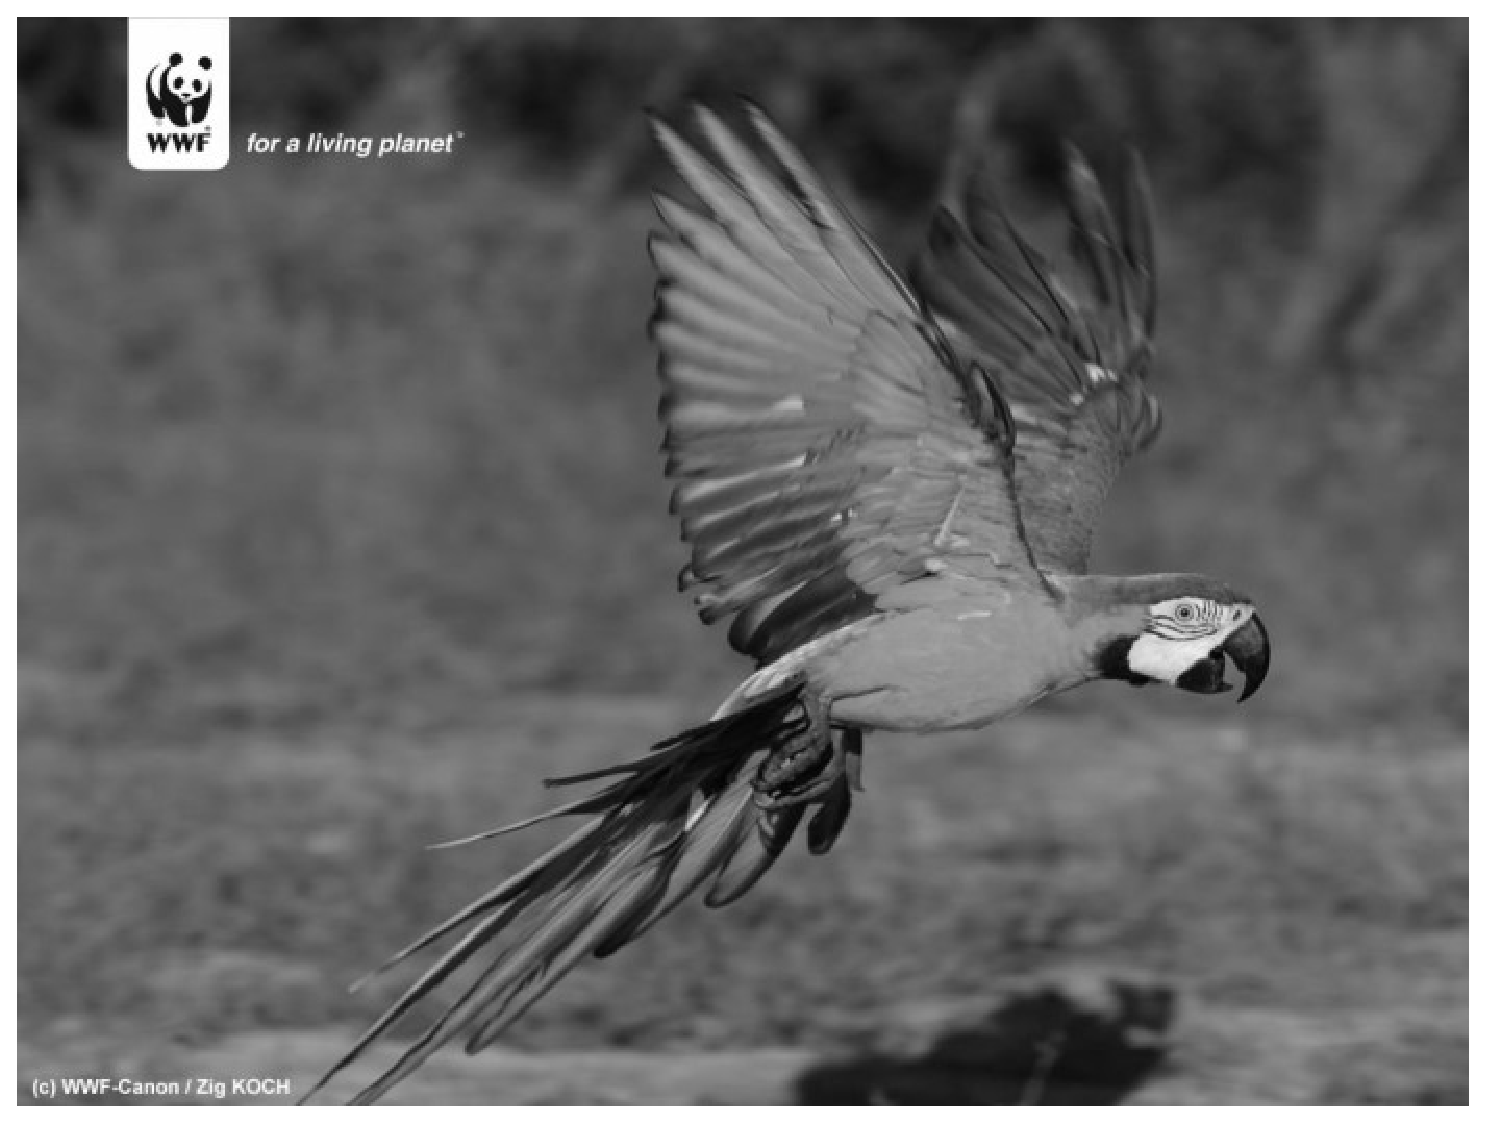
\includegraphics[width = 0.5 \linewidth]{ara_orig.eps}
      
      \caption{Image originale}
  \end{figure}

  \begin{figure}[!h]

    \begin{tabular}{cc}
    
      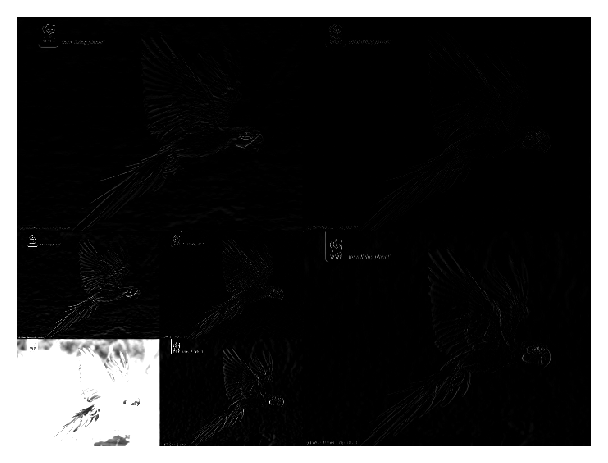
\includegraphics[width = 0.5 \linewidth]{ara_sqrt2.eps} &
      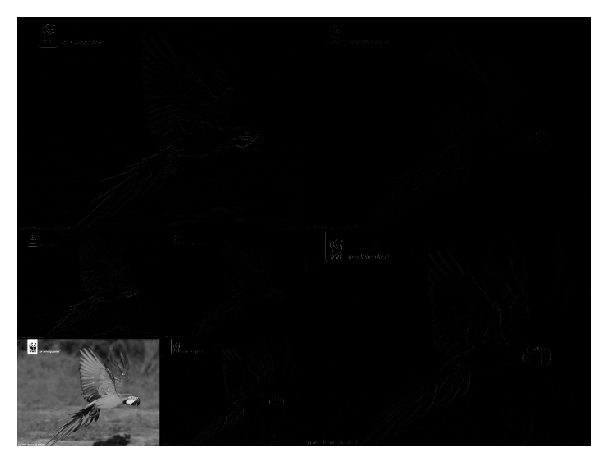
\includegraphics[width = 0.5 \linewidth]{ara_wt_V1.eps} \\	
      
    \end{tabular}
    
    \caption{Exemple de la diff\'{e}rence entre le choix du scalaire $\frac{1}{\sqrt{2}}$ (\`{a} gauche) 
	et du scalaire $\frac{1}{2}$ (\`{a} droite)}
    
  \end{figure}
  
  \paragraph{} On voit ainsi tr\`{e}s clairement que le scalaire $\frac{1}{2}$ permet de garder une bonne luminosit\'{e} de l'image originale.

\chapter{}

  \section*{Fichier $array.ml$}
  
    \begin{lstlisting}
let range n =
  let t = Array.make n 0 in
  for i = 1 to n - 1 do
    t.(i) <- i
  done;
  t

let ceil i d =
  if i mod d = 0 then i / d
  else i / d + 1

module type VECT =
  sig
    type 'a vect

    val vect_of_array : 'a array -> 'a vect
    val array_of_vect : 'a vect -> 'a array
    val length : 'a vect -> int
    val create : 'a -> int -> 'a vect
    val create_empty : 'a -> 'a vect
    val make_matrix : 'a -> int -> int -> 'a vect vect
    val alternate_id : int -> 'a -> ('a -> 'a) -> 'a vect
    val extend : 'a vect -> int -> 'a -> 'a vect

    val affect : 'a vect -> 'a -> int -> unit
    val value : 'a vect -> int -> 'a
    val reverse : 'a vect -> 'a vect
    val concat : 'a vect -> 'a vect -> 'a vect
    val sum : 'a vect -> 'a vect -> ('a -> 'a -> 'a) -> 'a vect
    val prod : 'a vect -> 'a vect -> ('a -> 'a -> 'a) -> 'a vect

    val sub_vect : 'a vect -> int -> int -> 'a vect
    val put_in : 'a vect -> 'a vect -> int -> unit
    val dilate : 'a vect -> int -> 'a -> 'a vect
    val extr_vect : 'a vect -> int -> int -> int -> 'a vect

    val filter : 'a vect -> 'a vect -> 'a vect -> ('a -> 'a -> 'a) -> ('a -> 'a -> 'a) -> ('a -> 'a) -> 'a -> 'a vect
  end;;
	
    \end{lstlisting}
\newpage
    \begin{lstlisting}

module Vect : VECT =
  struct
    type 'a vect = 'a array

    let vect_of_array t = t
    let array_of_vect v = v

    let length v = Array.length v
		
    let create x n = Array.make n x

    let create_empty x = Array.make 0 x

    let value v ind = v.(ind)

    let affect v x ind = v.(ind) <- x

    let make_matrix x n m = Array.make_matrix n m x

    let alternate_id n one opp =
      let v = create one n in
      for i = 0 to n - 1 do
	if i mod 2 = 1 then
	  affect v (opp one) i
      done; v

    let reverse v = 
      let n = length v in
      let v_rev = create (value v 0) n in
      for i = 0 to n - 1 do
	affect v_rev (value v (n - 1 - i)) i
      done; v_rev

    let concat v1 v2 = 
      let n = length v1 and p = length v2 in
      if n = 0 then v2
      else if p = 0 then v1
      else
	let v = create (value v1 0) (n + p) in
	for i = 1 to (n + p - 1) do
	  if i < n then 
	    affect v (value v1 i) i
	  else 
	    affect v (value v2 (i - n)) i
	done; v

    let sum v1 v2 sum_elem = 
      let n = length v1 in
      if not (n = length v2) then 
	failwith "Vect.sum"
      else
	let v = create (value v1 0) n in
	for i = 0 to n - 1 do
	  affect v (sum_elem (value v1 i) (value v2 i)) i
	done; v
	
    \end{lstlisting}
\newpage
    \begin{lstlisting}

    let prod v1 v2 prod_elem = 
      let n = length v1 in
      if not (n = length v2) then
	failwith "Vect.prod"
      else
	let v = create (value v1 0) n in
	for i = 0 to n - 1 do
	  affect v (prod_elem (value v1 i) (value v2 i)) i
	done; v

    let sub_vect v i j = 
      let v_sub = create (value v i) (j - i) in
      for k = 1 to j - i - 1 do
	affect v_sub (value v (k + i)) k
      done; v_sub

    let put_in v1 v2 i =
      let n = length v2 in
      if (i + n) > (length v1) then
	failwith "Vect.put_in"
      else
	for j = 0 to n - 1 do
	  affect v1 (value v2 j) (j + i)
	done

    let extend x m zero =
      let n = length x in
      if m = 0 then x
      else
	let y = create zero (n + m) in
	put_in y x 0;
	y

    let dilate v s zero = 
      let n = length v in
      let v_dil = create zero (n*s) in
      for i = 0 to n - 1 do
	affect v_dil (value v i) (s*i)
      done;
      v_dil
		
    let extr_vect v ind_beg diff_ind ind_end = 
      let n = ceil (ind_end - ind_beg) diff_ind in
      let v_ex = create (value v 0) n in
      let p = ref ind_beg and q = ref 0 in
      while !p < ind_end do
	affect v_ex (value v !p) !q;
	incr q; p := !p + diff_ind
      done; v_ex
	
    \end{lstlisting}
\newpage
    \begin{lstlisting}

    let filter b a x sum prod inv zero =
      let n = length x in
      let y = create (value x 0) n in
      let nb = length b in
			
      let b = (if n > nb then extend b (n - nb) zero else b) in	
			
      for i = 0 to n - 1 do
	let s = ref zero in
	for j = 0 to i do
	  s := sum !s (prod (value b j) (value x (i - j)))
	done;
	s := prod !s (inv (value a 0));
	affect y !s i
      done;
      y

  end

module type MATRIX =
  sig
    type 'a matrix

    val dim : 'a matrix -> (int * int)
    val create : 'a -> int -> int -> 'a matrix
    val matrix_of_vect : 'a Vect.vect -> 'a matrix

    val value : 'a matrix -> (int * int) -> 'a
    val affect : 'a matrix -> 'a -> (int * int) -> unit
    val vect : 'a matrix -> int -> 'a Vect.vect
    val affect_vect : 'a matrix -> 'a Vect.vect -> (int * int) -> unit
    val put_in : 'a matrix -> 'a matrix -> (int * int) -> unit
    val line : 'a matrix -> int -> 'a Vect.vect
    val affect_line : 'a matrix -> 'a Vect.vect -> (int * int) -> unit

    val sum : 'a matrix -> 'a matrix -> ('a -> 'a -> 'a) -> 'a matrix
    val prod_scal_cano : 'a matrix -> 'a matrix -> ('a -> 'a -> 'a) -> ('a -> 'a -> 'a) -> 'a -> 'a
    val norm_eucli : 'a matrix -> ('a -> 'a -> 'a) -> ('a -> 'a -> 'a) -> 'a -> 'a

    val extr_matrix : 'a matrix -> (int * int) -> (int * int) -> 'a matrix
  end;;

module Matrix : MATRIX =
  struct
    type 'a matrix = ('a Vect.vect) Vect.vect

    let value mat (i, j) = Vect.value (Vect.value mat i) j

    let affect mat x (i, j) = 
      let vect = Vect.value mat i in
      Vect.affect vect x j; Vect.affect mat vect i
		
    let dim mat = (Vect.length mat, Vect.length (Vect.value mat 0))
		
    let create x n m = Vect.make_matrix x n m 
	
    \end{lstlisting}
\newpage
    \begin{lstlisting}

    let matrix_of_vect v = Vect.create v 1

    let vect mat j = 
      let (n, m) = dim mat in
      let vect_mat = Vect.create (value mat (0, j)) n in
      for i = 1 to n - 1 do
	Vect.affect vect_mat (value mat (i, j)) i
      done; vect_mat

    let affect_vect mat vect (i, j) =
      for k = 0 to (Vect.length vect - 1) do
	affect mat (Vect.value vect k) (i + k, j)
      done

    let line mat i = Vect.value mat i

    let affect_line mat vect (i, ind_beg) =
      let line_mat = line mat i in
      Vect.put_in line_mat vect ind_beg;
      Vect.affect mat line_mat i

    let put_in mat1 mat2 (i, j) =
      for k = 0 to fst (dim mat2) - 1 do
	affect_line mat1 (line mat2 k) (i + k, j)
      done
		
    let sum mat1 mat2 sum_elem =
      let size = dim mat1 in
      if not (size = dim mat2) then
	failwith "Matrix.sum"
      else
	let mat = create (value mat1 (0, 0)) (fst size) (snd size) in
	for i = 0 to fst size - 1 do
	  affect_line mat (Vect.sum (line mat1 i) (line mat2 i) sum_elem) (i, 0)
	done; 
	mat

    let prod_scal_cano mat1 mat2 sum_elem prod_elem zero =
      let (n, m) = dim mat1 in
      if (n, m) <> dim mat2 then
	failwith "Matrix.prod_scal_cano"
      else
	let prod_scal = ref zero in
	for i = 0 to n - 1 do
	  for j = 0 to m - 1 do
	    prod_scal := sum_elem !prod_scal (prod_elem (value mat1 (i, j)) (value mat2 (i, j)))
	  done
	done;
	!prod_scal				

    let norm_eucli mat sum_elem prod_elem zero =
      prod_scal_cano mat mat sum_elem prod_elem zero
	
    \end{lstlisting}
\newpage
    \begin{lstlisting}

    let extr_matrix mat (i, j) (n2, m2) =
      let (n, m) = dim mat in
      if (i + n2 > n || j + m2 > m) then
	failwith "Matrix.extr_matrix";
      let mat_extr = create (value mat (i, j)) n2 m2 in
      for k = 0 to n2 - 1 do
	for l = 0 to m2 - 1 do
	  affect mat_extr (value mat (i + k, j + l)) (k, l)
	done
      done;
      mat_extr

  end;;

#use "bmp.ml"

module type PIXEL_MATRIX =
  sig
    type pixel
    type pixel_matrix
	
    val barycenter : pixel -> float

    val read_pixels : bitmapFileHeader -> bitmapInfoHeader -> in_channel -> pixel_matrix
    val write_pixels : out_channel -> pixel_matrix -> unit
    val read_bmp : string -> pixel_matrix
    val write_bmp : string -> pixel_matrix -> unit

    val intmatrix_of_matrix : float Matrix.matrix -> int Matrix.matrix

    val gray_levels : pixel_matrix -> float Matrix.matrix
    val pick_color : pixel -> int -> int
    val extr_uplet : pixel_matrix -> int -> float Matrix.matrix
    val red_filter : pixel_matrix -> float Matrix.matrix
    val blue_filter : pixel_matrix -> float Matrix.matrix
    val green_filter : pixel_matrix -> float Matrix.matrix
    val combine_filters : int Matrix.matrix -> int Matrix.matrix -> int Matrix.matrix -> pixel_matrix
  end;;

module Pixel_matrix : PIXEL_MATRIX =
  struct
    type pixel = (int * int * int)
    type pixel_matrix = pixel Matrix.matrix

    let barycenter (r, g, b) =
      ( (float_of_int r) +. (float_of_int g) +. (float_of_int b)) /. 3.
	
    \end{lstlisting}
\newpage
    \begin{lstlisting}
	    
    let read_pixels fh ih channel =
      let w = ih.biWidth
      and h = ih.biHeight in
      let offs = offset w in
      let m = Matrix.create (0, 0, 0) w h in
      for j = 0 to h - 1 do
	for i = 0 to w - 1 do
	  let b = input_byte channel in
	  let g = input_byte channel in
	  let r = input_byte channel in
	  Matrix.affect m (r, g, b) (i, j)
	done;
	for i = 1 to offs do
	  let _ = input_byte channel in ()
	done
      done;
      m

    let write_pixels channel m =
      let (w, h) = Matrix.dim m in
      let offs = offset w in
      for j = 0 to h - 1 do
	for i = 0 to w - 1 do
	  let r, g, b = Matrix.value m (i, j) in
	  output_byte channel b;
	  output_byte channel g;
	  output_byte channel r;
	done;
	for i = 1 to offs do
	  output_byte channel 0
	done
      done

    let read_bmp filename =
      let channel = open_in_bin filename in
      let fh = read_file_header channel in
      let ih = read_info_header channel in
      let m = read_pixels fh ih channel in
      close_in channel;
      m

    let write_bmp filename m =
      let channel = open_out_bin filename in
      let (w, h) = Matrix.dim m in
      let fh = make_file_header w h
      and ih = make_info_header w h in
      write_file_header channel fh;
      write_info_header channel ih;
      write_pixels channel m;
      close_out channel
	
    \end{lstlisting}
\newpage
    \begin{lstlisting}

    let intmatrix_of_matrix matrix =
      let (w, h) = Matrix.dim matrix in
      let intmatrix = Matrix.create 0 w h in
      for i = 0 to w - 1 do
	for j = 0 to h - 1 do
	  let matrix_i_j = Matrix.value matrix (i, j) in
	  if matrix_i_j > 255. then
	    Matrix.affect intmatrix 255 (i, j)
	  else if matrix_i_j < 0. then
	    Matrix.affect intmatrix 0 (i, j)
	  else
	    Matrix.affect intmatrix (int_of_float matrix_i_j) (i, j)
	done
      done;
      intmatrix

    let gray_levels m =
      let (w, h) = Matrix.dim m in
      let m1 = Matrix.create (0.) w h in
      for i = 0 to w - 1 do
	for j = 0 to h - 1 do
	  let p = Matrix.value m (i, j) in
	  let c = barycenter p in
	  Matrix.affect m1 c (i, j)
	done
      done;
      m1

    let pick_color (r, g, b) i =
      match i with
	| 1 -> r
	| 2 -> g
	| 3 -> b
	| _ -> failwith "Pixel_matrix.pick_uplet"

    let extr_uplet mat c = 
      let (w, h) = Matrix.dim mat in
      let m1 = Matrix.create (0.) w h in
      for i = 0 to w - 1 do
	for j = 0 to h - 1 do
	  let p = Matrix.value mat (i, j) in
	  let u = float_of_int (pick_color p c) in
	  Matrix.affect m1 u (i, j)
	done
      done;
      m1
	    
    let red_filter mat = extr_uplet mat 1
    let green_filter mat = extr_uplet mat 2
    let blue_filter mat = extr_uplet mat 3
	
    \end{lstlisting}
\newpage
    \begin{lstlisting}

    let combine_filters r_f g_f b_f =
      let (w, h) = Matrix.dim r_f in
      if (not ((w,h) = Matrix.dim g_f)) || (not ((w,h) = Matrix.dim b_f)) then 
	failwith "Pixel_matrix.combine_filters"
      else
	let m = Matrix.create (0, 0, 0) w h in
	for i = 0 to w - 1 do
	  for j = 0 to h - 1 do
	    let r = Matrix.value r_f (i, j)
	    and g = Matrix.value g_f (i, j)
	    and b = Matrix.value b_f (i, j)
	    in
	    Matrix.affect m (r, g, b) (i, j)
	  done
	done;
	m

  end
    \end{lstlisting}

  \section*{Fichier $fwt.ml$}

    \begin{lstlisting}
#use "array.ml"

let op x = -. x
let inv x = 1. /. x
let prod = ( *. )
let sum = ( +. )
let zero = 0.
let one = 1.
let two = sum one one
let vect_1 = Vect.vect_of_array [|one|]

let round_2 n =
  if n mod 2 = 0 then n/2
  else n/2 + 1

let rec pow x n = 
  if n = 0 then 1
  else 
    let y = pow x (n / 2) in
    if n mod 2 = 0 then
      y * y
    else 
      x * y * y

let normalise x (n, m) pow_2 =
  let offs_n = (if (n mod pow_2 = 0) then 0 else pow_2 - (n mod pow_2))
  and offs_m = (if (m mod pow_2 = 0) then 0 else pow_2 - (m mod pow_2)) in
  let y = Matrix.create zero (n + offs_n) (m + offs_m) in
  Matrix.put_in y x (0, 0);
  y, (n + offs_n, m + offs_m)
	
    \end{lstlisting}
\newpage
    \begin{lstlisting}

let denormalise x (n, m) =
  Matrix.extr_matrix x (0, 0) (n, m)

let aco f x =
  let n = Vect.length x
  and p = Vect.length f in
  let xpadded = ref (Vect.create_empty (Vect.value x 0)) in
  (if p < n then
    xpadded := (Vect.concat x (Vect.sub_vect x 0 p))
  else
    let z = Vect.create zero p in
    for i = 0 to p - 1 do
      let imod = (i mod n) in
      Vect.affect z (Vect.value x imod) i
    done;
    xpadded := (Vect.concat x z));
  let fflip = Vect.reverse f in
  let ypadded = Vect.filter fflip vect_1 !xpadded sum prod inv zero in
  Vect.sub_vect ypadded (p - 1) (n + p - 1)

let hi_up x g0 = 
  let tmp = ref (Vect.dilate x 2 zero) in
  let len_tmp = Vect.length !tmp - 1 in
  tmp := Vect.concat (Vect.create (Vect.value !tmp len_tmp) 1) 
	(Vect.sub_vect !tmp 0 len_tmp);
  aco g0 !tmp

let lo_conv x qmf =
  let d = aco qmf x in
  Vect.extr_vect d 0 2 (Vect.length d - 1)

let ico f x =
  let n = Vect.length x 
  and p = Vect.length f in
  let xpadded = ref (Vect.create (Vect.value x 0) 1) in
  (if p <= n then
    xpadded := (Vect.concat (Vect.sub_vect x (n - p) n) x)
  else
    let z = Vect.create zero p in
    for i = 0 to p - 1 do
      let imod = ( (p * n - p + i) mod n ) in
      Vect.affect z (Vect.value x imod) i
    done;
    xpadded := (Vect.concat z x));
  let ypadded = Vect.filter f vect_1 !xpadded sum prod inv zero in
  Vect.sub_vect ypadded p (n + p)

let hi_conv s qmf = 
  let s2 = Vect.concat (Vect.sub_vect s 1 (Vect.length s)) 
	  (Vect.create (Vect.value s 0) 1) in
  let d = ico qmf s2 in
  Vect.extr_vect d 0 2 (Vect.length d - 1)
	
    \end{lstlisting}
\newpage
    \begin{lstlisting}

let fwt sens x l h0 =
  let len_h0 = Vect.length h0 in 
  let g0 = Vect.prod (Vect.alternate_id len_h0 one op) h0 prod in

  if sens = 0 then
  (let wc, (n, m) = normalise x (Matrix.dim x) (pow 2 l) in
  let nc = ref n
  and mc = ref m in

  for jsqual = 1 to l do
    for ix = 0 to !nc - 1 do
      let row = Vect.sub_vect (Matrix.line wc ix) 0 !mc in
      Matrix.affect_line wc (lo_conv row h0) (ix, 0);
      Matrix.affect_line wc (hi_conv row g0) (ix, (!mc / 2));
    done;

    for iy = 0 to !mc - 1 do
      let row = Vect.sub_vect (Matrix.vect wc iy) 0 !nc in
      Matrix.affect_vect wc (hi_conv row g0) (!nc / 2, iy);
      Matrix.affect_vect wc (lo_conv row h0) (0, iy);
    done;

    nc := !nc / 2; mc := !mc / 2
  done; wc)

  else
    (let (n, m) = Matrix.dim x in
    let pow_2 = pow 2 (l - 1) in
    let nc = ref (n / pow_2)
    and mc = ref (m / pow_2) in

    for jsqual = 1 to l do
      for iy = 0 to !mc - 1 do
	Matrix.affect_vect x (Vect.sum 
		(ico h0 (Vect.dilate 
			    (Vect.sub_vect (Matrix.vect x iy) 0 (!nc / 2)) 
			    2 zero)) 
		(hi_up (Vect.sub_vect (Matrix.vect x iy) (!nc / 2) !nc) g0) 
		sum) (0, iy)
      done;

      for ix = 0 to !nc - 1 do
	Matrix.affect_line x (Vect.sum 
		(ico h0 (Vect.dilate 
			    (Vect.sub_vect (Matrix.line x ix) 0 (!mc / 2)) 
			    2 zero)) 
		(hi_up (Vect.sub_vect (Matrix.line x ix) (!mc / 2) !mc) g0) 
		sum) (ix, 0)
      done;

      nc := !nc * 2; mc := !mc * 2;
    done; x)

    \end{lstlisting}

\newpage
    
  \section*{Fichier $compression\_wt.ml$}
  
    \begin{lstlisting}
#use "array.ml";;
#use "fwt.ml";;

let abs x =
  if x < zero then op x
  else x

let abs2 x =
  if x < 0 then - x
  else x

let haar_filter = Vect.prod_scal (Vect.vect_of_array [|1. ; 1.|]) 2. ( /. );;
let haar_filter2 = Vect.vect_of_array [|1. ; 1.|];;

let decompo_wt_matrix img_m it =
  fwt 0 img_m it haar_filter;;

let decompo_wt img it =
  let img_matrix = Pixel_matrix.read_bmp img in
  let gray_matrix = Pixel_matrix.gray_levels img_matrix in
  let decompo = decompo_wt_matrix gray_matrix it in
  decompo;;
		
let rec calc_indice_div it (n, m) =
  if it = 0 then
    (n, m)
  else
    calc_indice_div (it - 1) (n / 2, m / 2)

let rec calc_indice_mult it (n, m) =
  if it = 0 then
    (n, m)
  else
    calc_indice_mult (it - 1) (n * 2, m * 2)

let txt_of_matrix mat it filename =
  let (n, m) = Matrix.dim mat in
  let (size_n, size_m) = calc_indice_div it (n, m) in
  let extr_mat = Matrix.extr_matrix mat (0, 0) (size_n, size_m) in
  let file = open_out filename in
  output_string file ((string_of_int it) ^ "\n");
  for i = 0 to n - 1 do
    for j = 0 to m - 1 do
      let mat_i_j = Matrix.value mat (i, j) in
      if (i >= size_n || j >= size_m) && mat_i_j <> 0 then
	let str = (string_of_int i) ^ " " ^ (string_of_int j) ^ 
		  " " ^ (string_of_int mat_i_j) ^ "\n" in
	output_string file str
    done
  done;
  close_out file;
  extr_mat
	
    \end{lstlisting}
\newpage
    \begin{lstlisting}

let decompo_line line =
  let tab = Array.make 3 0 in
  let n = String.length line in
  let str = ref "" in
  let j = ref 0 in
  for i = 0 to n - 1 do
    if line.[i] <> ' ' then
      (str := !str ^ (String.make 1 line.[i]);
      if i = n - 1 then
	tab.(!j) <- int_of_string !str)
    else
      (tab.(!j) <- int_of_string !str;
      str := "";
      incr j)
  done;
  (tab.(0), tab.(1), tab.(2)) 

let matrix_of_txt mat filename =
  let file = open_in filename in
  let mult = int_of_string (input_line file) in
  let (size_n, size_m) = Matrix.dim mat in
  let (n, m) = calc_indice_mult mult (size_n, size_m) in
  
  let complete_mat = Matrix.create 0. n m in
  Matrix.put_in complete_mat mat (0, 0); 
  
  let end_of_file = ref false in

  while (not !end_of_file) do
    try
      let line = input_line file in
      let (i, j, value) = decompo_line line in
      Matrix.affect complete_mat (float_of_int value) (i, j)
    with
      | End_of_file -> end_of_file := true
  done;
  close_in file;
  
  (complete_mat, mult);;

let compresser_img img it filename_target =
  let mat = decompo_wt img it in
  let intmat = Pixel_matrix.intmatrix_of_matrix mat in
  let extr_mat = txt_of_matrix intmat it filename_target in
  Pixel_matrix.write_bmp (filename_target ^ ".bmp") 
      (Pixel_matrix.combine_filters extr_mat extr_mat extr_mat);;

let decompresser_img img file target =
  let mat = Pixel_matrix.read_bmp img in
  let gray_mat = Pixel_matrix.gray_levels mat in
  let (mat_recomp, it) = matrix_of_txt gray_mat file in
  let decomp = fwt 1 mat_recomp it haar_filter2 in
  let intdecomp = Pixel_matrix.intmatrix_of_matrix decomp in
  let combine = Pixel_matrix.combine_filters intdecomp intdecomp intdecomp in
  Pixel_matrix.write_bmp target combine;;
	
    \end{lstlisting}
\newpage
    \begin{lstlisting}

let error img it i =
  let mat = Pixel_matrix.read_bmp img in
  let original = Pixel_matrix.gray_levels mat in
  let comp = decompo_wt_matrix original it in

  let intcomp = Pixel_matrix.intmatrix_of_matrix comp in
  let extr = txt_of_matrix intcomp it ("text" ^ (string_of_int (i + 1))) in
  
  let pixextr = Pixel_matrix.combine_filters extr extr extr in
  let extrfloat = Pixel_matrix.gray_levels pixextr in

  let (recomp, _) = matrix_of_txt extrfloat ("text" ^ (string_of_int (i + 1))) in

  let decomp = fwt 1 recomp it haar_filter2 in

  let denorm_decomp = denormalise decomp (Matrix.dim original) in

  let intoriginal = Pixel_matrix.intmatrix_of_matrix original
  and intdecomp = Pixel_matrix.intmatrix_of_matrix denorm_decomp in

  let mat_diff = Matrix.sum intoriginal intdecomp ( - ) in
  Matrix.norm_eucli mat_diff ( + ) ( * ) 0
    \end{lstlisting}

\chapter{}

  \section*{Fichier $bmp.ml$}
  
    \begin{lstlisting}
#load "graphics.cma";;
open Graphics;;

type word  = int;;
type dword = int;;

type bitmapFileHeader = {
  bfType      : string;
  bfSize      : dword;
  bfReserved1 : word;
  bfReserved2 : word;
  bfOffBits   : dword;
};;

type bitmapInfoHeader = {
  biSize          : dword;
  biWidth         : dword;
  biHeight        : dword;
  biPlanes        : word;
  biBitCount      : word;
  biCompression   : dword;
  biSizeImage     : dword;
  biXPelsPerMeter : dword;
  biYPelsPerMeter : dword;
  biClrUsed       : dword;
  biClrImportant  : dword;
};;
let read_type channel = 
  let s = "  " in
  s.[0] <- input_char channel;
  s.[1] <- input_char channel;
  s;;
 
let write_type channel = 
  output_char channel 'B';
  output_char channel 'M';;
	
    \end{lstlisting}
\newpage
    \begin{lstlisting}

let read_dword channel =
  let a = input_byte channel in
  let b = input_byte channel in
  let c = input_byte channel in
  let d = input_byte channel in
  (d lsl 24) lor (c lsl 16) lor (b lsl 8) lor a;;

let write_dword channel x =
  let a = x lsr 24
  and b = (x lsr 16) land 255
  and c = (x lsr 8) land 255
  and d = x land 255 in
  output_byte channel d;
  output_byte channel c;
  output_byte channel b;
  output_byte channel a;;
  
let read_word channel =
  let a = input_byte channel in
  let b = input_byte channel in
  (b lsl 8) lor a;;

let write_word channel x =
  let c = (x lsr 8) land 255
  and d = x land 255 in
  output_byte channel d;
  output_byte channel c;;

let read_file_header channel =
  let t = read_type channel in
  let sz = read_dword channel in
  let r1 = read_word channel in
  let r2 = read_word channel in
  let off = read_dword channel in
  {
    bfType = t;
    bfSize = sz;
    bfReserved1 = r1;
    bfReserved2 = r2;
    bfOffBits = off;
  };;
  
let write_file_header channel fh =
  write_type channel;
  write_dword channel fh.bfSize;
  write_word channel fh.bfReserved1;
  write_word channel fh.bfReserved2;
  write_dword channel fh.bfOffBits;;
	
    \end{lstlisting}
\newpage
    \begin{lstlisting}

let read_info_header channel =
  let sz = read_dword channel in
  let w = read_dword channel in
  let h = read_dword channel in
  let pl = read_word channel in
  let bc = read_word channel in
  let compr = read_dword channel in
  let szim = read_dword channel in
  let xpm = read_dword channel in
  let ypm = read_dword channel in
  let clru = read_dword channel in
  let clri = read_dword channel in
  {
    biSize = sz;
    biWidth = w;
    biHeight = h;
    biPlanes = pl;
    biBitCount = bc;
    biCompression = compr;
    biSizeImage = szim;
    biXPelsPerMeter= xpm;
    biYPelsPerMeter= ypm;
    biClrUsed = clru;
    biClrImportant = clri;
  };;
  
let write_info_header channel ih =
  write_dword channel ih.biSize;
  write_dword channel ih.biWidth;
  write_dword channel ih.biHeight;
  write_word channel ih.biPlanes;
  write_word channel ih.biBitCount;
  write_dword channel ih.biCompression;
  write_dword channel ih.biSizeImage;
  write_dword channel ih.biXPelsPerMeter;
  write_dword channel ih.biYPelsPerMeter;
  write_dword channel ih.biClrUsed;
  write_dword channel ih.biClrImportant;;

let offset w =
  let r = (3 * w) mod 4 in
  if r = 0 then 0
  else 4 - r;;

let make_file_header w h = 
  let off = offset w in
  {
    bfType = "BM";
    bfSize = (w + off) * h * 3 + 54;
    bfReserved1  = 0;
    bfReserved2 = 0;
    bfOffBits = 54;
  };;
	
    \end{lstlisting}
\newpage
    \begin{lstlisting}
  
let make_info_header w h = 
  let off = offset w in
  {
    biSize = 40;
    biWidth = w;
    biHeight  = h;
    biPlanes  = 1;
    biBitCount = 24;
    biCompression = 0;
    biSizeImage = (w + off) * h * 3;
    biXPelsPerMeter = 0;
    biYPelsPerMeter = 0;
    biClrUsed = 0;
    biClrImportant = 0;
  };;
    \end{lstlisting}


\end{document}          

%      \'{e}crit par Philippe Carr\'{e}, professeur de l'universit\'{e} de Poitiers et responsable de l'\'{e}quipe Icones, 
%      et R\'{e}mi Cornillet, \'{e}tudiant \`{a} l'ENS de Rennes.